		Firstly, it is easy to find that phenanthrene belongs to the point group $\mathscr{C}_{\rm 2h}$, whose character table is listed below.
		\begin{center}
		\setlength{\abovecaptionskip}{-0.1em}
		\captionof{table}{The character table for the $\mathscr{C}_{\rm 2h}$ point group.}
		\begin{tabular}{ccccc}\hline
	$\mathscr{C}_{\rm 2h}$ & $E$ & $C_2$ & $i$ & $\sigma_h$ \\ \hline
			$A_g$	&	1	&	1	&	1	&	1	\\
			$B_g$	&	1	&	-1	&	1	&	-1	\\
			$A_u$	&	1	&	1	&	-1	&	-1	\\
			$B_u$ 	&	1	&	-1	&	-1	&	1	\\ \hline
		\end{tabular}
		\setlength{\belowcaptionskip}{-0.2em}
		\end{center}
		
		Besides, its all nontrivial symmetry elements are shown in \Figref{fig:sym_elem_6}.
		\begin{center}
		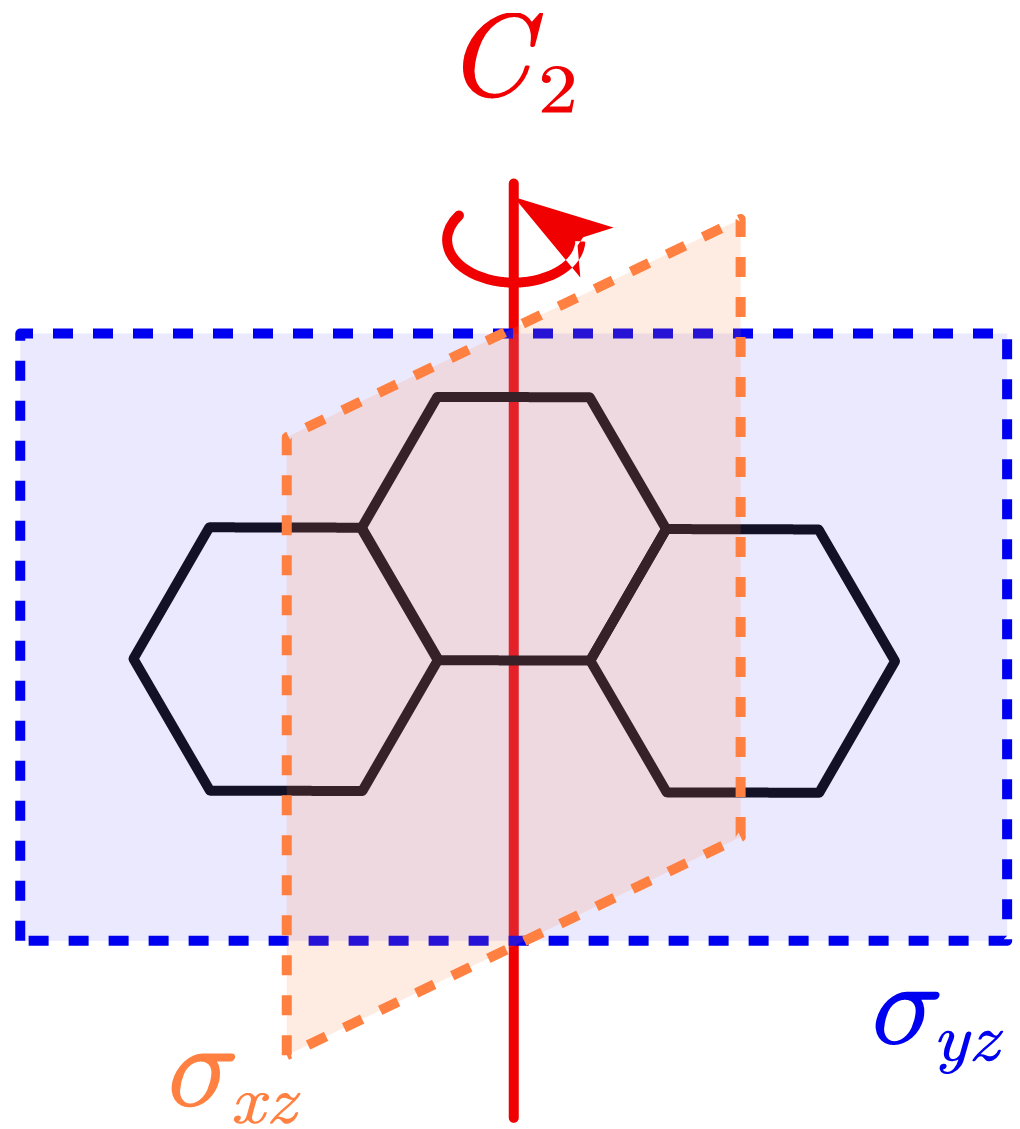
\includegraphics[scale=1.0]{./structures/exercise_1/phenanthrene/999.png}
		\captionof{figure}{All nontrivial symmetry elements of phenanthrene.}\label{fig:sym_elem_6}
		\end{center}	
		
		Secondly, we mark all carbon atoms as shown in \Figref{fig:phenanthrene}.
		\begin{center}
		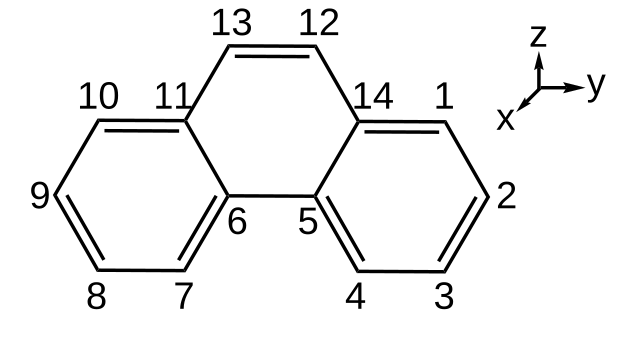
\includegraphics[scale=1.0]{./structures/exercise_1/phenanthrene/0.png}
		\setlength{\abovecaptionskip}{-0.3em}
		\captionof{figure}{The label of carbon atoms in phenanthrene.}\label{fig:phenanthrene}
		\setlength{\belowcaptionskip}{-0.8em}
		\end{center}				
		
		For $\pi$-electron atomic orbitals' representation $\Gamma^{\rm AO}$, its following characters is listed below.
		\begin{center}
		\setlength{\abovecaptionskip}{-0.3em}
		\captionof{table}{The character of the $\pi$-electron atomic orbitals' representation $\Gamma^{\rm AO}$.}
		\begin{tabular}{ccccc}\hline
	$\mathscr{C}_{\rm 2v}$	& $E$ & $C_2$ &	$\sigma_{xz}$	& $\sigma_{yz}$ \\ \hline
	$\chi^{\AO}(C_i)$	&	14	&	0	&	0	&	-14	\\ \hline
		\end{tabular}\vspace*{-0.5em}
		\end{center}
		Relevant reduction coefficients are
		\begin{equation*}
		a_1 = 0, \quad a_2 = 7, \quad b_1 = 7, \quad b_2 = 0.
		\end{equation*}
		Thus, we obtain
		\begin{equation*}
			\Gamma^{\AO} = 7\Gamma^{A_2} \oplus 7\Gamma^{B_1}.
		\end{equation*}
		We conclude that there are seven basis functions in the irreducible representation $\Gamma^{A_2}$ and $\Gamma^{B_1}$, respectively. Thus, to describe the effect of $O_R$, seven suitable $2 \orbp_z$ atomic orbitals $\phi_i$ is enough.
		
		Thirdly, we inspect the transformation of $\phi_i$ under $O_R$ for the phenanthrene, whose information is recorded below. We have to list up to seven $2 \orbp_z$ functions in current case.
		\begin{center}
		\setlength{\abovecaptionskip}{0em}
		\captionof{table}{Transformation of $\phi_i$ under $O_R$ for the phenanthrene.}
		\begin{tabular}{ccccc}\hline
	$\mathscr{C}_{\rm 2v}$ & $E$ & $C_2$ &	$\sigma_{xz}$	& $\sigma_{yz}$	\\ \hline
			$\phi_1$	&	$\phi_1$	&	$-\phi_{10}$	&	$\phi_{10}$	&	$-\phi_1$	\\
			$\phi_2$	&	$\phi_2$	&	$-\phi_9$	&	$\phi_9$	&	$-\phi_2$		\\
			$\phi_3$	&	$\phi_3$	&	$-\phi_8$	&	$\phi_8$	&	$-\phi_3$		\\
			$\phi_4$	&	$\phi_4$	&	$-\phi_7$	&	$\phi_7$	&	$-\phi_4$		\\ 
			$\phi_5$	&	$\phi_5$	&	$-\phi_6$	&	$\phi_6$	&	$-\phi_5$		\\ 
			$\phi_{11}$	&	$\phi_{11}$	&	$-\phi_{14}$	&	$\phi_{14}$	&	$-\phi_{11}$		\\
			$\phi_{12}$	&	$\phi_{12}$	&	$-\phi_{13}$	&	$\phi_{13}$	&	$-\phi_{12}$		\\ \hline
		\end{tabular}
		\end{center}
		
		Fourthly, it's time to discuss situations in different irreducible representation. 
		
		For the irreducible representation $\Gamma^{A_2}$,
		\begin{align*}
		P^{A_2}\phi_1 &= \sum_{R} \chi^{A_2}(R) O_R \phi_1 = 2(\phi_1-\phi_{10}) , \\
		P^{A_2}\phi_2 &= \sum_{R} \chi^{A_2}(R) O_R \phi_2 = 2(\phi_2-\phi_9) ,	\\
		P^{A_2}\phi_3 &= \sum_{R} \chi^{A_2}(R) O_R \phi_3 = 2(\phi_3-\phi_8) ,	\\
		P^{A_2}\phi_4 &= \sum_{R} \chi^{A_2}(R) O_R \phi_4 = 2(\phi_4-\phi_7) ,	\\
		P^{A_2}\phi_5 &= \sum_{R} \chi^{A_2}(R) O_R \phi_5 = 2(\phi_5-\phi_6) ,	\\
		P^{A_2}\phi_6 &= \sum_{R} \chi^{A_2}(R) O_R \phi_6 = 2(\phi_{11}-\phi_{14}) ,	\\
		P^{A_2}\phi_7 &= \sum_{R} \chi^{A_2}(R) O_R \phi_7 = 2(\phi_{12}-\phi_{13}) .
		\end{align*}
		It is easy to find that they are mutually orthogonal. They can be normalized to
		\begin{align*}
		\phi^\prime_1 &= \frac{1}{\sqrt{2}} (\phi_1-\phi_{10}) , \\
		\phi^\prime_2 &= \frac{1}{\sqrt{2}} (\phi_2-\phi_9) , \\
		\phi^\prime_3 &= \frac{1}{\sqrt{2}} (\phi_3-\phi_8) , \\
		\phi^\prime_4 &= \frac{1}{\sqrt{2}} (\phi_4-\phi_7) , \\
		\phi^\prime_5 &= \frac{1}{\sqrt{2}} (\phi_5-\phi_6) , \\
		\phi^\prime_6 &= \frac{1}{\sqrt{2}} (\phi_{11}-\phi_{14}) , \\		
		\phi^\prime_7 &= \frac{1}{\sqrt{2}} (\phi_{12}-\phi_{13}) .
		\end{align*}
		
		Then, the effective Hamitonian matrix elements for $\pi$ electrons can be calculated,
		\begin{equation*}
			\Hp_{A_2} = \begin{pmatrix}
\alpha&\beta&	0	&	0	&		0	&	-\beta 	&	0	\\
\beta&\alpha&\beta	&	0	&		0	&	0	&	0	\\
0	&\beta	&\alpha	&\beta	&		0	&	0	&	0	\\
0	&	0	&\beta	&\alpha	&	\beta	&	0	&	0	\\
0	&	0	&	0	&\beta	&\alpha-\beta&	-\beta	&	0\\
-\beta&	0	&	0	&	0	& -\beta	&	\alpha	&	\beta \\
0	&	0	&	0	&	0	&	0		&	\beta	&\alpha-\beta\\
			\end{pmatrix}					
		\end{equation*}
		Next,
		\begin{align*}
			\det(\Hp_{A_2}-\varepsilon^\pi \Sp_{A_2}) = \beta^7 ( x^7 - 2x^6 - 6x^5 + 11x^4 + 9x^3 -15x^2 -4x +5 ) = 0,
		\end{align*}
		where
		\begin{equation*}
			x \equiv \frac{\alpha - \varepsilon^\pi}{\beta}.
		\end{equation*}
		
		Obviously, it is hard to solve this equation analytically. We have to apply numerical solution. The polynomial function $y=x^7 - 2x^6 - 6x^5 + 11x^4 + 9x^3 -15x^2 -4x +5$ in the closed interval $[-2.5, 2.5]$ can be plotted as shown in \Figref{fig:poly_a2}.
		
		\begin{center}
		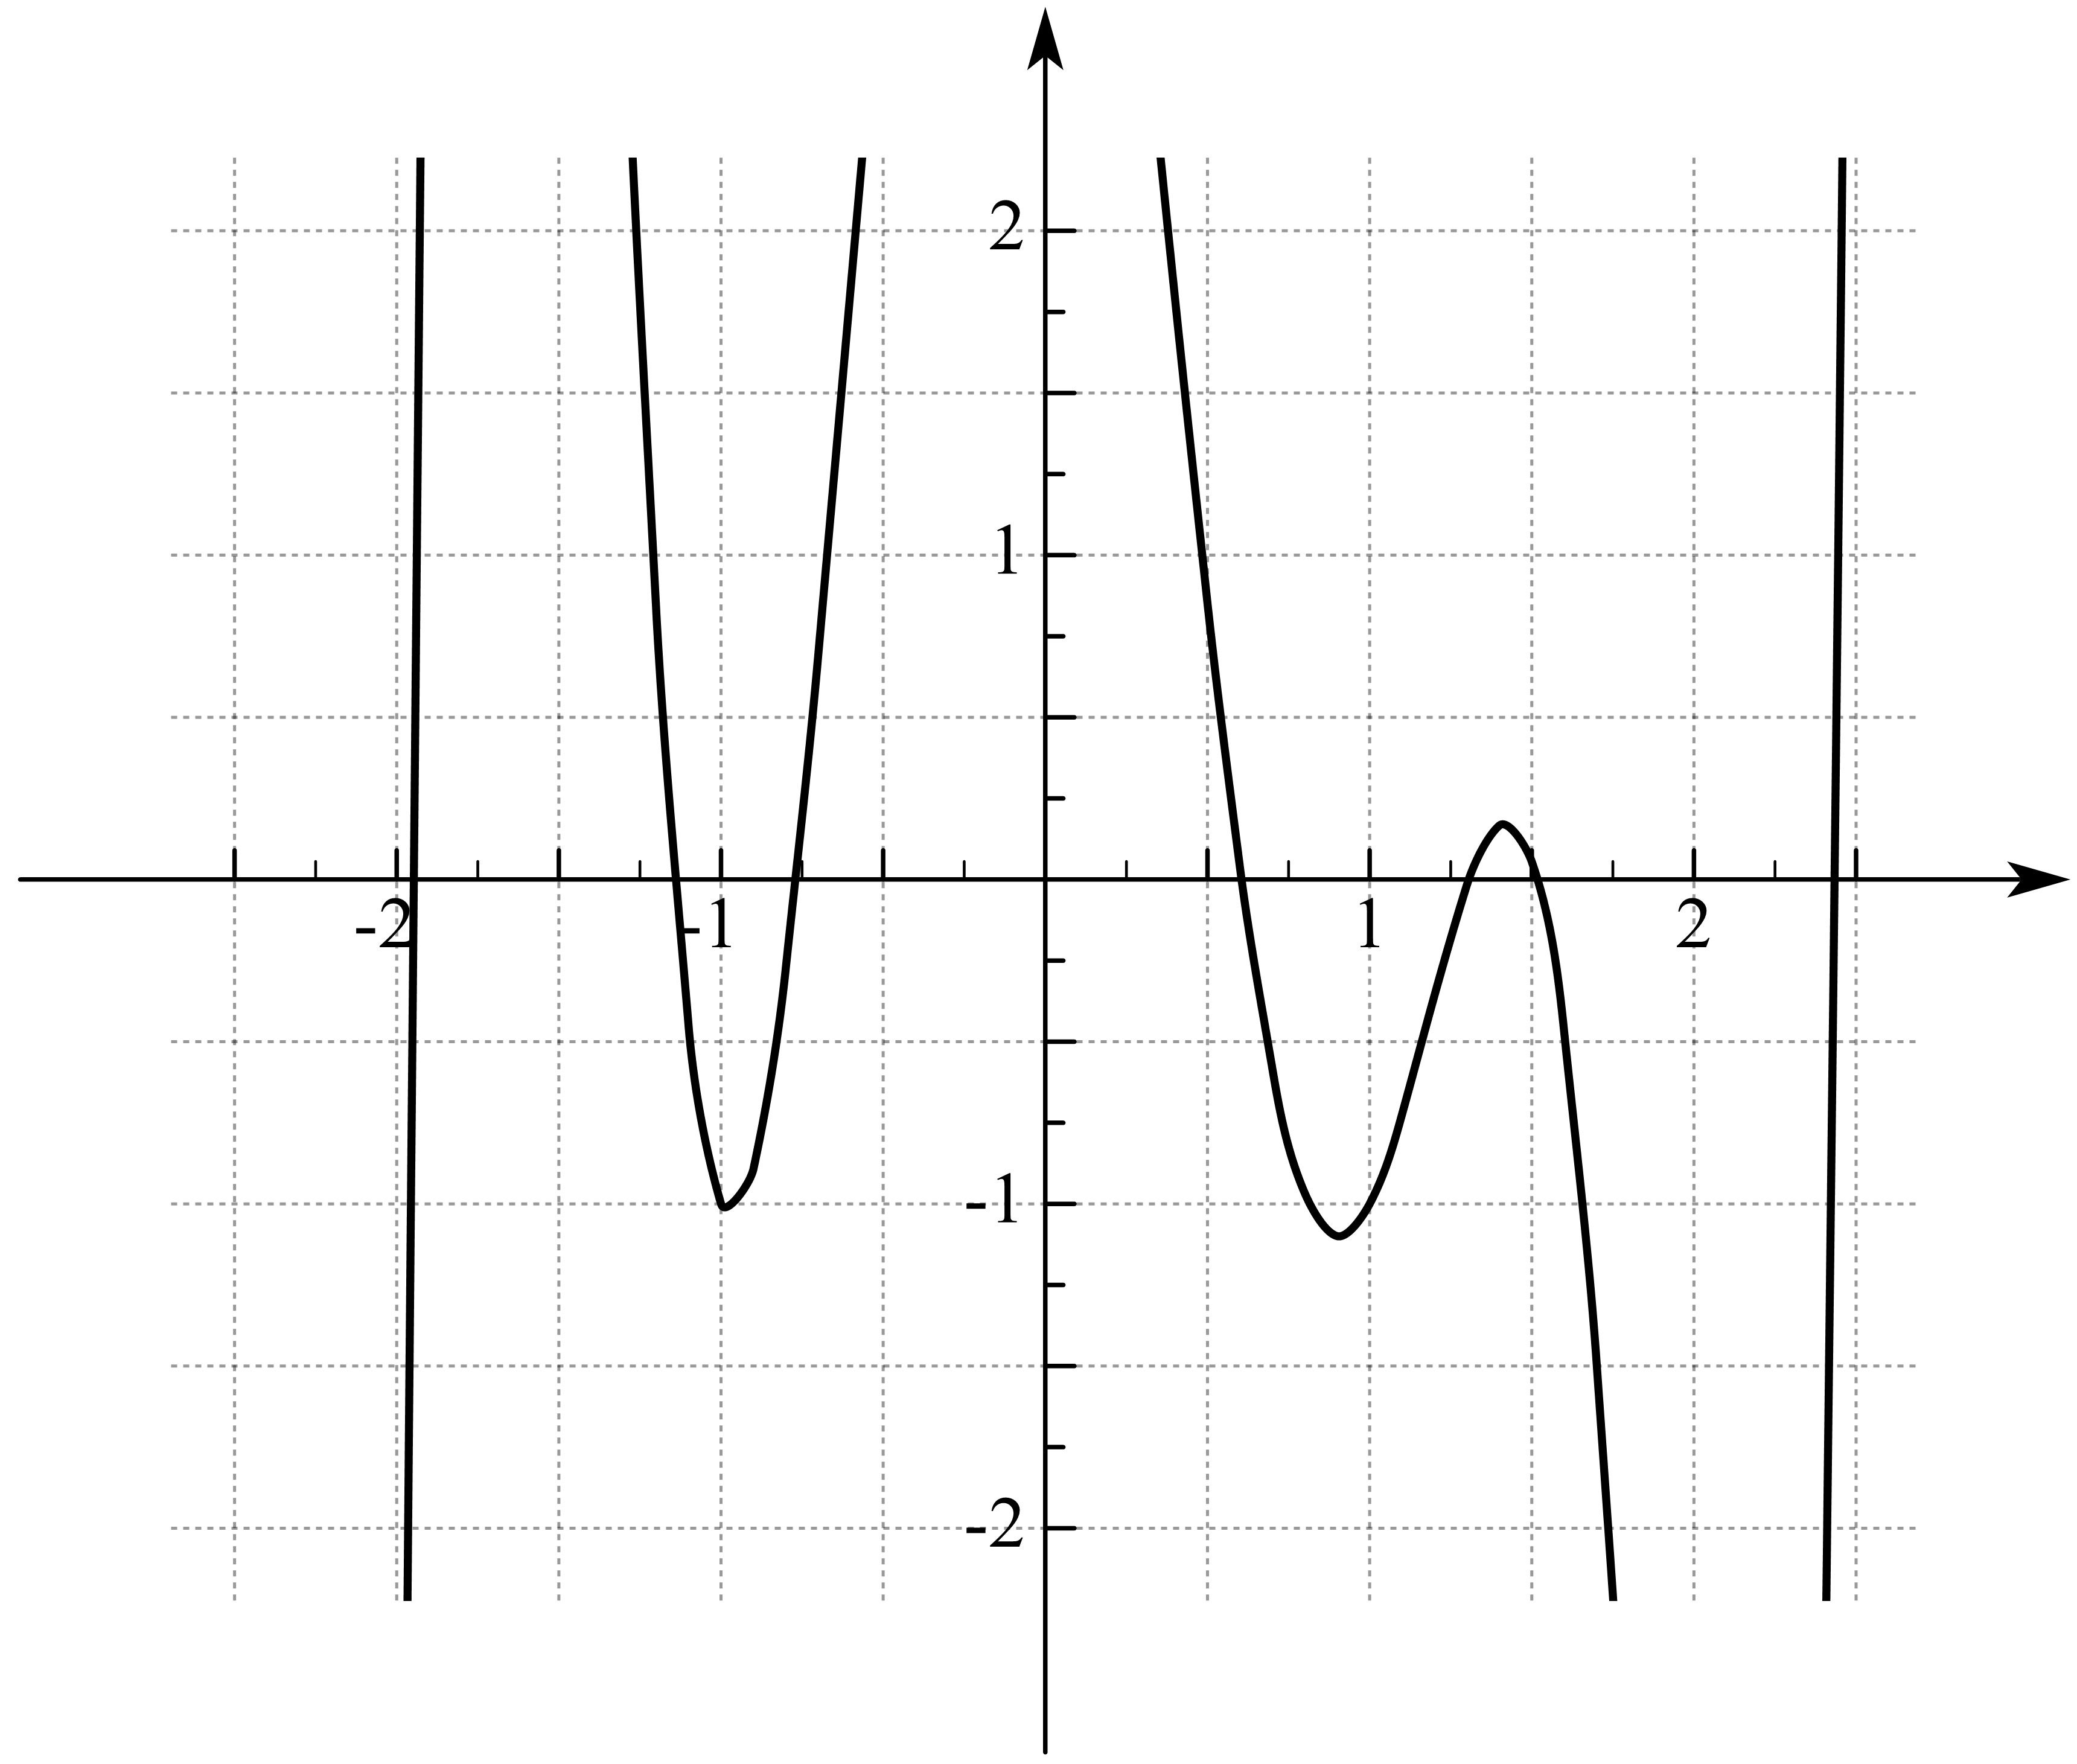
\includegraphics[scale=1]{./structures/exercise_1/phenanthrene/997.png}
		\captionof{figure}{The diagram of function $y=x^7 - 2x^6 - 6x^5 + 11x^4 + 9x^3 -15x^2 -4x +5$ in the closed interval $[-2.5, 2.5]$.}\label{fig:poly_a2}
		\end{center}				
		There are seven roots,
		\begin{center}
		\begin{tabular}{llll}
			$x_1 \approx -1.95063$, & $x_2 \approx -1.14238$, & $x_3 \approx -0.769052$, & $x_4 \approx 0.605225 $, \\
			$x_5 \approx 1.30580$, & $x_6\approx 1.51627$, & $x_7 \approx 2.43476$. &
		\end{tabular}
		\end{center}
		which equal to	
		\begin{align}
			\varepsilon_1 &= \alpha - x_1 \beta \approx \alpha + 1.95063 \beta , \\
			\varepsilon_2 &= \alpha - x_2 \beta\approx \alpha + 1.14238 \beta , \\
			\varepsilon_3 &= \alpha - x_3 \beta\approx \alpha + 0.769052 \beta , \\
			\varepsilon_4 &= \alpha - x_4 \beta\approx \alpha - 0.605225 \beta , \\
			\varepsilon_5 &= \alpha - x_5 \beta\approx \alpha - 1.30580 \beta , \\
			\varepsilon_6 &= \alpha - x_6 \beta\approx \alpha - 1.51627 \beta , \\
			\varepsilon_7 &= \alpha - x_7 \beta\approx \alpha - 2.43476 \beta .
		\end{align}
		
		For $\Hp_{B_2}-\varepsilon^\pi_1 \Sp_{B_2}$, its reduced row echelon form is
		\begin{equation*}
			\begin{pmatrix}
			1 & 0 & 0 & 0 & 0 & 0 & 2.991107 \\
			0 & 1 & 0 & 0 & 0 & 0 & 2.884044 \\
			0 & 0 & 1 & 0 & 0 & 0 & 2.634595 \\
			0 & 0 & 0 & 1 & 0 & 0 & 2.255077 \\
			0 & 0 & 0 & 0 & 1 & 0 & 1.764225 \\
			0 & 0 & 0 & 0 & 0 & 1 & -2.950499 \\
			0 & 0 & 0 & 0 & 0 & 0 & 0 \\
			\end{pmatrix},
		\end{equation*}
		which means
		\begin{equation*}
			\Phi_1 = 2.991107 \phi^\prime_1 + 2.884044 \phi^\prime_2 + 2.634595 \phi^\prime_3 + 2.255077 \phi^\prime_4 + 1.764225 \phi^\prime_5 - 2.950499 \phi^\prime_6 - 1.000000 \phi^\prime_7.
		\end{equation*}
		The sum of squares of coefficients is
		\begin{equation*}
			\sum_{i=1}^7 c^2_{1,i} = 42.1088.
		\end{equation*}
		Thus, we know
		\begin{align}
			\Phi^\pi_1 &= \frac{1}{\sqrt{\sum_{i=1}^7 c^2_{1,i}}} \Phi_1 \approx 0.154104 \Phi_1 \notag \\
			&\approx 0.46094 \phi^\prime_1 + 0.44444 \phi^\prime_2 + 0.40600 \phi^\prime_3 + 0.34752 \phi^\prime_4 + 0.27187 \phi^\prime_5 - 0.45468 \phi^\prime_6 - 0.15410 \phi^\prime_7 \notag \\
			&\approx 0.32594 \phi_1 + 0.31427 \phi_2 + 0.28709 \phi_3 + 0.24573 \phi_4 + 0.19224 \phi_5  \notag \\
			&\hspace*{4em} - 0.19224\phi_6 - 0.24573 \phi_7 - 0.28709 \phi_8 - 0.31427 \phi_9  -0.32594\phi_{10} \notag \\
			&\hspace*{4em}- 0.32151 \phi_{11} - 0.10897 \phi_{12} + 0.10897 \phi_{13} + 0.32151 \phi_{14} .
		\end{align}	
		
		Similarly, we can obtain other eigenvalues and their eigenfunctions. Their intermediate and final results are listed.
		\begin{itemize}
		
		
		\item $\varepsilon_2 \approx \alpha + 1.14238 \beta$
		
		The original eigenfunction is
		\begin{equation*}
			\Phi_2 = 1.19554 \phi^\prime_1 - 0.77669 \phi^\prime_2 -2.08281 \phi^\prime_3 -1.60267 \phi^\prime_4 +0.25195 \phi^\prime_5 - 2.14244 \phi^\prime_6 - 1.00000 \phi^\prime_7.
		\end{equation*}
		
		The sum of coefficients is
		\begin{equation*}
			\sum_{i} c^2_{2,i} = 14.5927.
		\end{equation*}

		The normalized eigenfunction is
		\begin{align}
			\Phi^\pi_2 &\approx 0.261777 \Phi_2 \notag \\
			&\approx 0.31296 \phi^\prime_1 - 0.20332 \phi^\prime_2 -0.54523 \phi^\prime_3 -0.41954 \phi^\prime_4 + 0.06596 \phi^\prime_5 - 0.56084 \phi^\prime_6 - 0.26178 \phi^\prime_7 \notag \\
			&\approx 0.22130 \phi_1 -0.14377 \phi_2 -0.38544 \phi_3 -0.29666 \phi_4 + 0.04664 \phi_5  \notag \\
			&\hspace*{4em} - 0.04664\phi_6 +0.29666 \phi_7 +0.38544 \phi_8 +0.14377 \phi_9  -0.22130 \phi_{10} \notag \\
			&\hspace*{4em}- 0.39658 \phi_{11} - 0.18510 \phi_{12} + 0.18510 \phi_{13} + 0.39658 \phi_{14} .
		\end{align}
		
		
		\item $\varepsilon_3 \approx \alpha + 0.769052 \beta$
		
		The original eigenfunction is
		\begin{equation*}
			\Phi_3 = 2.70354 \phi^\prime_1 + 3.84820 \phi^\prime_2 +0.25592 \phi^\prime_3 -3.65138 \phi^\prime_4 - 3.06402 \phi^\prime_5 + 1.76903 \phi^\prime_6 + 1.00000 \phi^\prime_7.
		\end{equation*}
		
		The sum of coefficients is
		\begin{equation*}
			\sum_{i} c^2_{3,i} = 49.0335.
		\end{equation*}
		
		The normalized eigenfunction is
		\begin{align}
			\Phi^\pi_3 &\approx 0.142808 \Phi_3 \notag \\
			&\approx 0.38609 \phi^\prime_1 + 0.54955 \phi^\prime_2 +0.03655 \phi^\prime_3 -0.52145 \phi^\prime_4 - 0.43757 \phi^\prime_5 + 0.25263 \phi^\prime_6 + 0.14281 \phi^\prime_7 \notag \\
			&\approx 0.27301\phi_1 +0.38858 \phi_2 +0.02584 \phi_3 -0.36872 \phi_4 -0.30941 \phi_5  \notag \\
			&\hspace*{4em} +0.30941 \phi_6 + 0.36872 \phi_7 -0.02584 \phi_8 -0.38858 \phi_9 -0.27301 \phi_{10} \notag \\
			&\hspace*{4em} +0.17864 \phi_{11} +0.10098 \phi_{12} -0.10098\phi_{13} -0.17864 \phi_{14} .
		\end{align}
		
		
		\item $\varepsilon_4 \approx \alpha - 0.605225 \beta$
		\begin{equation*}
			\Phi_4 = 0.81967 \phi^\prime_1 -0.10131 \phi^\prime_2 -0.75836 \phi^\prime_3 + 0.56029 \phi^\prime_4 + 0.41926 \phi^\prime_5 + 0.39478 \phi^\prime_6 + 1.00000 \phi^\prime_7.
		\end{equation*}
		\begin{equation*}
			\sum_{i} c^2_{4,i} = 2.90277.
		\end{equation*}
		\begin{align}
			\Phi^\pi_4 &\approx 0.586940 \Phi_4 \notag \\
			&\approx 0.48110 \phi^\prime_1 - 0.05946 \phi^\prime_2 -0.44511 \phi^\prime_3 +0.32885 \phi^\prime_4 + 0.24608 \phi^\prime_5 + 0.23171 \phi^\prime_6 + 0.58694 \phi^\prime_7 \notag \\
			&\approx 0.34019 \phi_1 -0.04205 \phi_2 -0.31474 \phi_3 + 0.23253 \phi_4 + 0.17400 \phi_5  \notag \\
			&\hspace*{4em} -0.17400 \phi_6 -0.23253 \phi_7 +0.31474 \phi_8 +0.04205 \phi_9 -0.34019 \phi_{10} \notag \\
			&\hspace*{4em} +0.16384 \phi_{11} + 0.41503 \phi_{12} -0.41503 \phi_{13} -0.16384\phi_{14} .
		\end{align}
		
		
		\item $\varepsilon_5 \approx \alpha -1.30580 \beta$
		
		The original eigenfunction is
		\begin{equation*}
			\Phi_5 = 3.45516 \phi^\prime_1 - 4.20593 \phi^\prime_2 + 2.03694 \phi^\prime_3 + 1.54608 \phi^\prime_4 - 4.05582 \phi^\prime_5 + 0.30582 \phi^\prime_6 - 1.00000 \phi^\prime_7.
		\end{equation*}
		
		The sum of coefficients is
		\begin{equation*}
			\sum_{i} c^2_{5,i} = 53.7106.
		\end{equation*}
		
		The normalized eigenfunction is
		\begin{align}
			\Phi^\pi_5 &\approx 0.136449 \Phi_5 \notag \\
			&\approx 0.47145 \phi^\prime_1 -0.57389 \phi^\prime_2 +0.27794 \phi^\prime_3 + 0.21096 \phi^\prime_4 - 0.55341 \phi^\prime_5 + 0.04173 \phi^\prime_6 - 0.13644 \phi^\prime_7 \notag \\
			&\approx 0.33337 \phi_1 -0.40580 \phi_2 +0.19653 \phi_3 + 0.14917 \phi_4 - 0.39132 \phi_5  \notag \\
			&\hspace*{4em} +0.39132 \phi_6 -0.14917 \phi_7 -0.19653 \phi_8 +0.40580 \phi_9 -0.33337 \phi_{10} \notag \\
			&\hspace*{4em} + 0.02951 \phi_{11} - 0.09648 \phi_{12} + 0.09648 \phi_{13} - 0.02951 \phi_{14} .
		\end{align}
		
		
		\item $\varepsilon_6 \approx \alpha -1.51627 \beta$
		
		The original eigenfunction is
		\begin{equation*}
			\Phi_6 = 0.04360 \phi^\prime_1 + 0.45017 \phi^\prime_2 -0.72618 \phi^\prime_3 +0.65091 \phi^\prime_4 -0.26078 \phi^\prime_5 + 0.51628 \phi^\prime_6 - 1.00000 \phi^\prime_7.
		\end{equation*}
		
		The sum of coefficients is
		\begin{equation*}
			\sum_{i} c^2_{6,i} = 2.49013.
		\end{equation*}
		
		The normalized eigenfunction is
		\begin{align}
			\Phi^\pi_6 &\approx 0.633708 \Phi_6 \notag \\
			&\approx 0.02763 \phi^\prime_1 + 0.28528 \phi^\prime_2 -0.46018 \phi^\prime_3 + 0.41249 \phi^\prime_4 - 0.16526 \phi^\prime_5 + 0.32717 \phi^\prime_6 - 0.63371 \phi^\prime_7 \notag \\
			&\approx 0.01954 \phi_1 +0.20172 \phi_2 - 0.32540 \phi_3 +0.29167 \phi_4 -0.11686 \phi_5  \notag \\
			&\hspace*{4em} +0.11686 \phi_6 -0.29167 \phi_7 + 0.32540\phi_8 -0.20172 \phi_9 - 0.01954 \phi_{10} \notag \\
			&\hspace*{4em} + 0.23134 \phi_{11} -0.44810 \phi_{12} +0.44810 \phi_{13} - 0.23134  \phi_{14} .
		\end{align}
		
		
		\item $\varepsilon_7 \approx \alpha -2.43476 \beta$
		
		The original eigenfunction is
		\begin{equation*}
			\Phi_7 = 0.83768 \phi^\prime_1 - 0.60476 \phi^\prime_2 +0.63476 \phi^\prime_3 - 0.94073 \phi^\prime_4 + 1.65569 \phi^\prime_5 + 1.43479 \phi^\prime_6 - 1.00000 \phi^\prime_7.
		\end{equation*}
		
		The sum of coefficients is
		\begin{equation*}
			\sum_{i} c^2_{7,i} = 8.15527.
		\end{equation*}
		
		The normalized eigenfunction is
		\begin{align}
			\Phi^\pi_7 &\approx 0.350171 \Phi_7 \notag \\
			&\approx 0.29333 \phi^\prime_1 - 0.21177 \phi^\prime_2 +0.22228 \phi^\prime_3 -0.32942 \phi^\prime_4 + 0.57978 \phi^\prime_5 + 0.50242 \phi^\prime_6 - 0.35017 \phi^\prime_7 \notag \\
			&\approx 0.20742 \phi_1 -0.14974 \phi_2 + 0.15717 \phi_3 -0.23293\phi_4 + 0.40996\phi_5  \notag \\
			&\hspace*{4em} -0.40996 \phi_6 +0.23293\phi_7 - 0.15717\phi_8 +0.14974 \phi_9 -0.20742 \phi_{10} \notag \\
			&\hspace*{4em} +0.35527 \phi_{11} -0.24761 \phi_{12} +0.24761 \phi_{13} -0.35527  \phi_{14} .
		\end{align}
		
		\end{itemize}
		
		In conclusion, for the irreducible representation $\Gamma^{A_2}$, relevant results are listed below.
		\begin{center}
		\setlength{\abovecaptionskip}{0em}
		\captionof{table}{The H{\"u}ckel MOs in the irreducible representation $\Gamma^{A_2}$ of phenanthrene.}
		\begin{tabular}{ccccccccc}\hline
		order & eigenvalue & \multicolumn{7}{c}{eigenfunction} \\ \hline
	\multirow{4}*{1}	&	\multirow{4}*{$\alpha+1.951\beta$}	& $c_1$ & $c_2$ & $c_3$ & $c_4$ & $c_5$ & $c_6$ & $c_7$\\\cline{3-9}
& & 0.3259 & 0.3143 & 0.2871 & 0.2457 & 0.1922 & -0.1922 & -0.2457 \\ \cline{3-9}
& & $c_8$ & $c_9$ & $c_{10}$ & $c_{11}$ & $c_{12}$ & $c_{13}$ & $c_{14}$\\\cline{3-9}
& & -0.2871 & -0.3143 & -0.3259 & -0.3215 & -0.1090 & 0.1090 & 0.3215 \\ \hline
	\multirow{4}*{2}	&	\multirow{4}*{$\alpha+1.142\beta$}	& $c_1$ & $c_2$ & $c_3$ & $c_4$ & $c_5$ & $c_6$ & $c_7$\\\cline{3-9}
& & 0.2213 & -0.1438 & -0.3855 & -0.2967 & 0.0466 & -0.0466 & 0.2967 \\ \cline{3-9}
& & $c_8$ & $c_9$ & $c_{10}$ & $c_{11}$ & $c_{12}$ & $c_{13}$ & $c_{14}$\\\cline{3-9}
& & 0.3855 & 0.1438 & -0.2213 & -0.3966 & -0.1851 & 0.1851 & 0.3966 \\ \hline
	\multirow{4}*{3}	&	\multirow{4}*{$\alpha+0.769\beta$}	& $c_1$ & $c_2$ & $c_3$ & $c_4$ & $c_5$ & $c_6$ & $c_7$\\\cline{3-9}
& & 0.2730 & 0.3886 & 0.0258 & -0.3687 & -0.3094 & 0.3094 & 0.3687 \\ \cline{3-9}
& & $c_8$ & $c_9$ & $c_{10}$ & $c_{11}$ & $c_{12}$ & $c_{13}$ & $c_{14}$\\\cline{3-9}
& & -0.0258 & -0.3886 & -0.2730 & 0.1786 & 0.1010 & -0.1010 & -0.1786 \\ \hline
\multirow{4}*{4}	&	\multirow{4}*{$\alpha-0.605\beta$}	& $c_1$ & $c_2$ & $c_3$ & $c_4$ & $c_5$ & $c_6$ & $c_7$\\\cline{3-9}
& & 0.3402 & -0.0420 & -0.3147 & 0.2325 & 0.1740 & -0.1740 & -0.2325 \\ \cline{3-9}
& & $c_8$ & $c_9$ & $c_{10}$ & $c_{11}$ & $c_{12}$ & $c_{13}$ & $c_{14}$\\\cline{3-9}
& & 0.3147 & 0.0420 & -0.3402 & 0.1638 & 0.4150 & -0.4150 & -0.1638 \\ \hline
\multirow{4}*{5}	&	\multirow{4}*{$\alpha-1.306\beta$}	& $c_1$ & $c_2$ & $c_3$ & $c_4$ & $c_5$ & $c_6$ & $c_7$\\\cline{3-9}
& & 0.3334 & -0.4058 & 0.1965 & 0.1492 & -0.3913 & 0.3913 & -0.1492 \\ \cline{3-9}
& & $c_8$ & $c_9$ & $c_{10}$ & $c_{11}$ & $c_{12}$ & $c_{13}$ & $c_{14}$\\\cline{3-9}
& & -0.1965 & 0.4058 & -0.3334 & 0.0295 & -0.0965 & 0.0965 & -0.0295 \\ \hline
\multirow{4}*{6}	&	\multirow{4}*{$\alpha-1.516\beta$}	& $c_1$ & $c_2$ & $c_3$ & $c_4$ & $c_5$ & $c_6$ & $c_7$\\\cline{3-9}
& & 0.0195 & 0.2017 & -0.3254 & 0.2917 & -0.1169 & 0.1169 & -0.2917 \\ \cline{3-9}
& & $c_8$ & $c_9$ & $c_{10}$ & $c_{11}$ & $c_{12}$ & $c_{13}$ & $c_{14}$\\\cline{3-9}
& & 0.3254 & -0.2017 & -0.0195 & 0.2313 & -0.4481 & 0.4481 & -0.2313 \\ \hline
\multirow{4}*{7}	&	\multirow{4}*{$\alpha-2.435\beta$}	& $c_1$ & $c_2$ & $c_3$ & $c_4$ & $c_5$ & $c_6$ & $c_7$\\\cline{3-9}
& & 0.2074 & -0.1497 & 0.1572 & -0.2329 & 0.4100 & -0.4100 & 0.2329 \\ \cline{3-9}
& & $c_8$ & $c_9$ & $c_{10}$ & $c_{11}$ & $c_{12}$ & $c_{13}$ & $c_{14}$\\\cline{3-9}
& & -0.1572 & 0.1497 & -0.2074 & 0.3553 & -0.2476 & 0.2476 & -0.3553 \\ \hline
		\end{tabular}
		\end{center}
		
		For the irreducible representation $\Gamma^{B_1}$,
		\begin{align*}
		P^{B_1}\phi_1 &= \sum_{R} \chi^{B_1}(R) O_R \phi_1 = 2(\phi_1 +\phi_{10}) , \\
		P^{B_1}\phi_2 &= \sum_{R} \chi^{B_1}(R) O_R \phi_2 = 2(\phi_2+\phi_9) ,	\\
		P^{B_1}\phi_3 &= \sum_{R} \chi^{B_1}(R) O_R \phi_3 = 2(\phi_3+\phi_8) ,	\\
		P^{B_1}\phi_4 &= \sum_{R} \chi^{B_1}(R) O_R \phi_4 = 2(\phi_4+\phi_7) ,	\\
		P^{B_1}\phi_5 &= \sum_{R} \chi^{B_1}(R) O_R \phi_5 = 2(\phi_5+\phi_6) ,	\\
		P^{B_1}\phi_6 &= \sum_{R} \chi^{B_1}(R) O_R \phi_6 = 2(\phi_{11}+\phi_{14}) ,	\\
		P^{B_1}\phi_7 &= \sum_{R} \chi^{B_1}(R) O_R \phi_7 = 2(\phi_{12}+\phi_{13}) .
		\end{align*}
		It is easy to find that they are mutually orthogonal. They can be normalized to
		\begin{align*}
		\phi^\prime_8 &= \frac{1}{\sqrt{2}} (\phi_1+\phi_{10}) , \\
		\phi^\prime_9 &= \frac{1}{\sqrt{2}} (\phi_2+\phi_9) , \\
		\phi^\prime_{10} &= \frac{1}{\sqrt{2}} (\phi_3+\phi_8) , \\
		\phi^\prime_{11} &= \frac{1}{\sqrt{2}} (\phi_4+\phi_7) , \\
		\phi^\prime_{12} &= \frac{1}{\sqrt{2}} (\phi_5+\phi_6) , \\
		\phi^\prime_{13} &= \frac{1}{\sqrt{2}} (\phi_{11}+\phi_{14}) , \\		
		\phi^\prime_{14} &= \frac{1}{\sqrt{2}} (\phi_{12}+\phi_{13}) .
		\end{align*}
		
		Then, the effective Hamitonian matrix elements for $\pi$ electrons can be calculated,
		\begin{equation*}
			\Hp_{B_1} = \begin{pmatrix}
\alpha&\beta&	0	&	0	&		0	&	\beta 	&	0	\\
\beta&\alpha&\beta	&	0	&		0	&	0	&	0	\\
0	&\beta	&\alpha	&\beta	&		0	&	0	&	0	\\
0	&	0	&\beta	&\alpha	&	\beta	&	0	&	0	\\
0	&	0	&	0	&\beta	&\alpha+\beta&	\beta	&	0\\
\beta&	0	&	0	&	0	& \beta		&	\alpha	&	\beta \\
0	&	0	&	0	&	0	&	0		&	\beta	&\alpha+\beta\\
			\end{pmatrix}					
		\end{equation*}
		Next,
		\begin{align*}
			\det(\Hp_{B_1}-\varepsilon^\pi \Sp_{B_1}) = \beta^7 ( x^7 + 2x^6 - 6x^5 - 11x^4 + 9x^3 +15x^2 -4x -5 ) = 0.
		\end{align*}
		
		We also apply numerical approach to solve $x^7 + 2x^6 - 6x^5 - 11x^4 + 9x^3 +15x^2 -4x -5 = 0$. The function $y=x^7 + 2x^6 - 6x^5 - 11x^4 + 9x^3 +15x^2 -4x -5$ in the closed interval $[-2.5, 2.5]$ is plotted as shown in \Figref{fig:poly_b1}.
		\begin{center}
		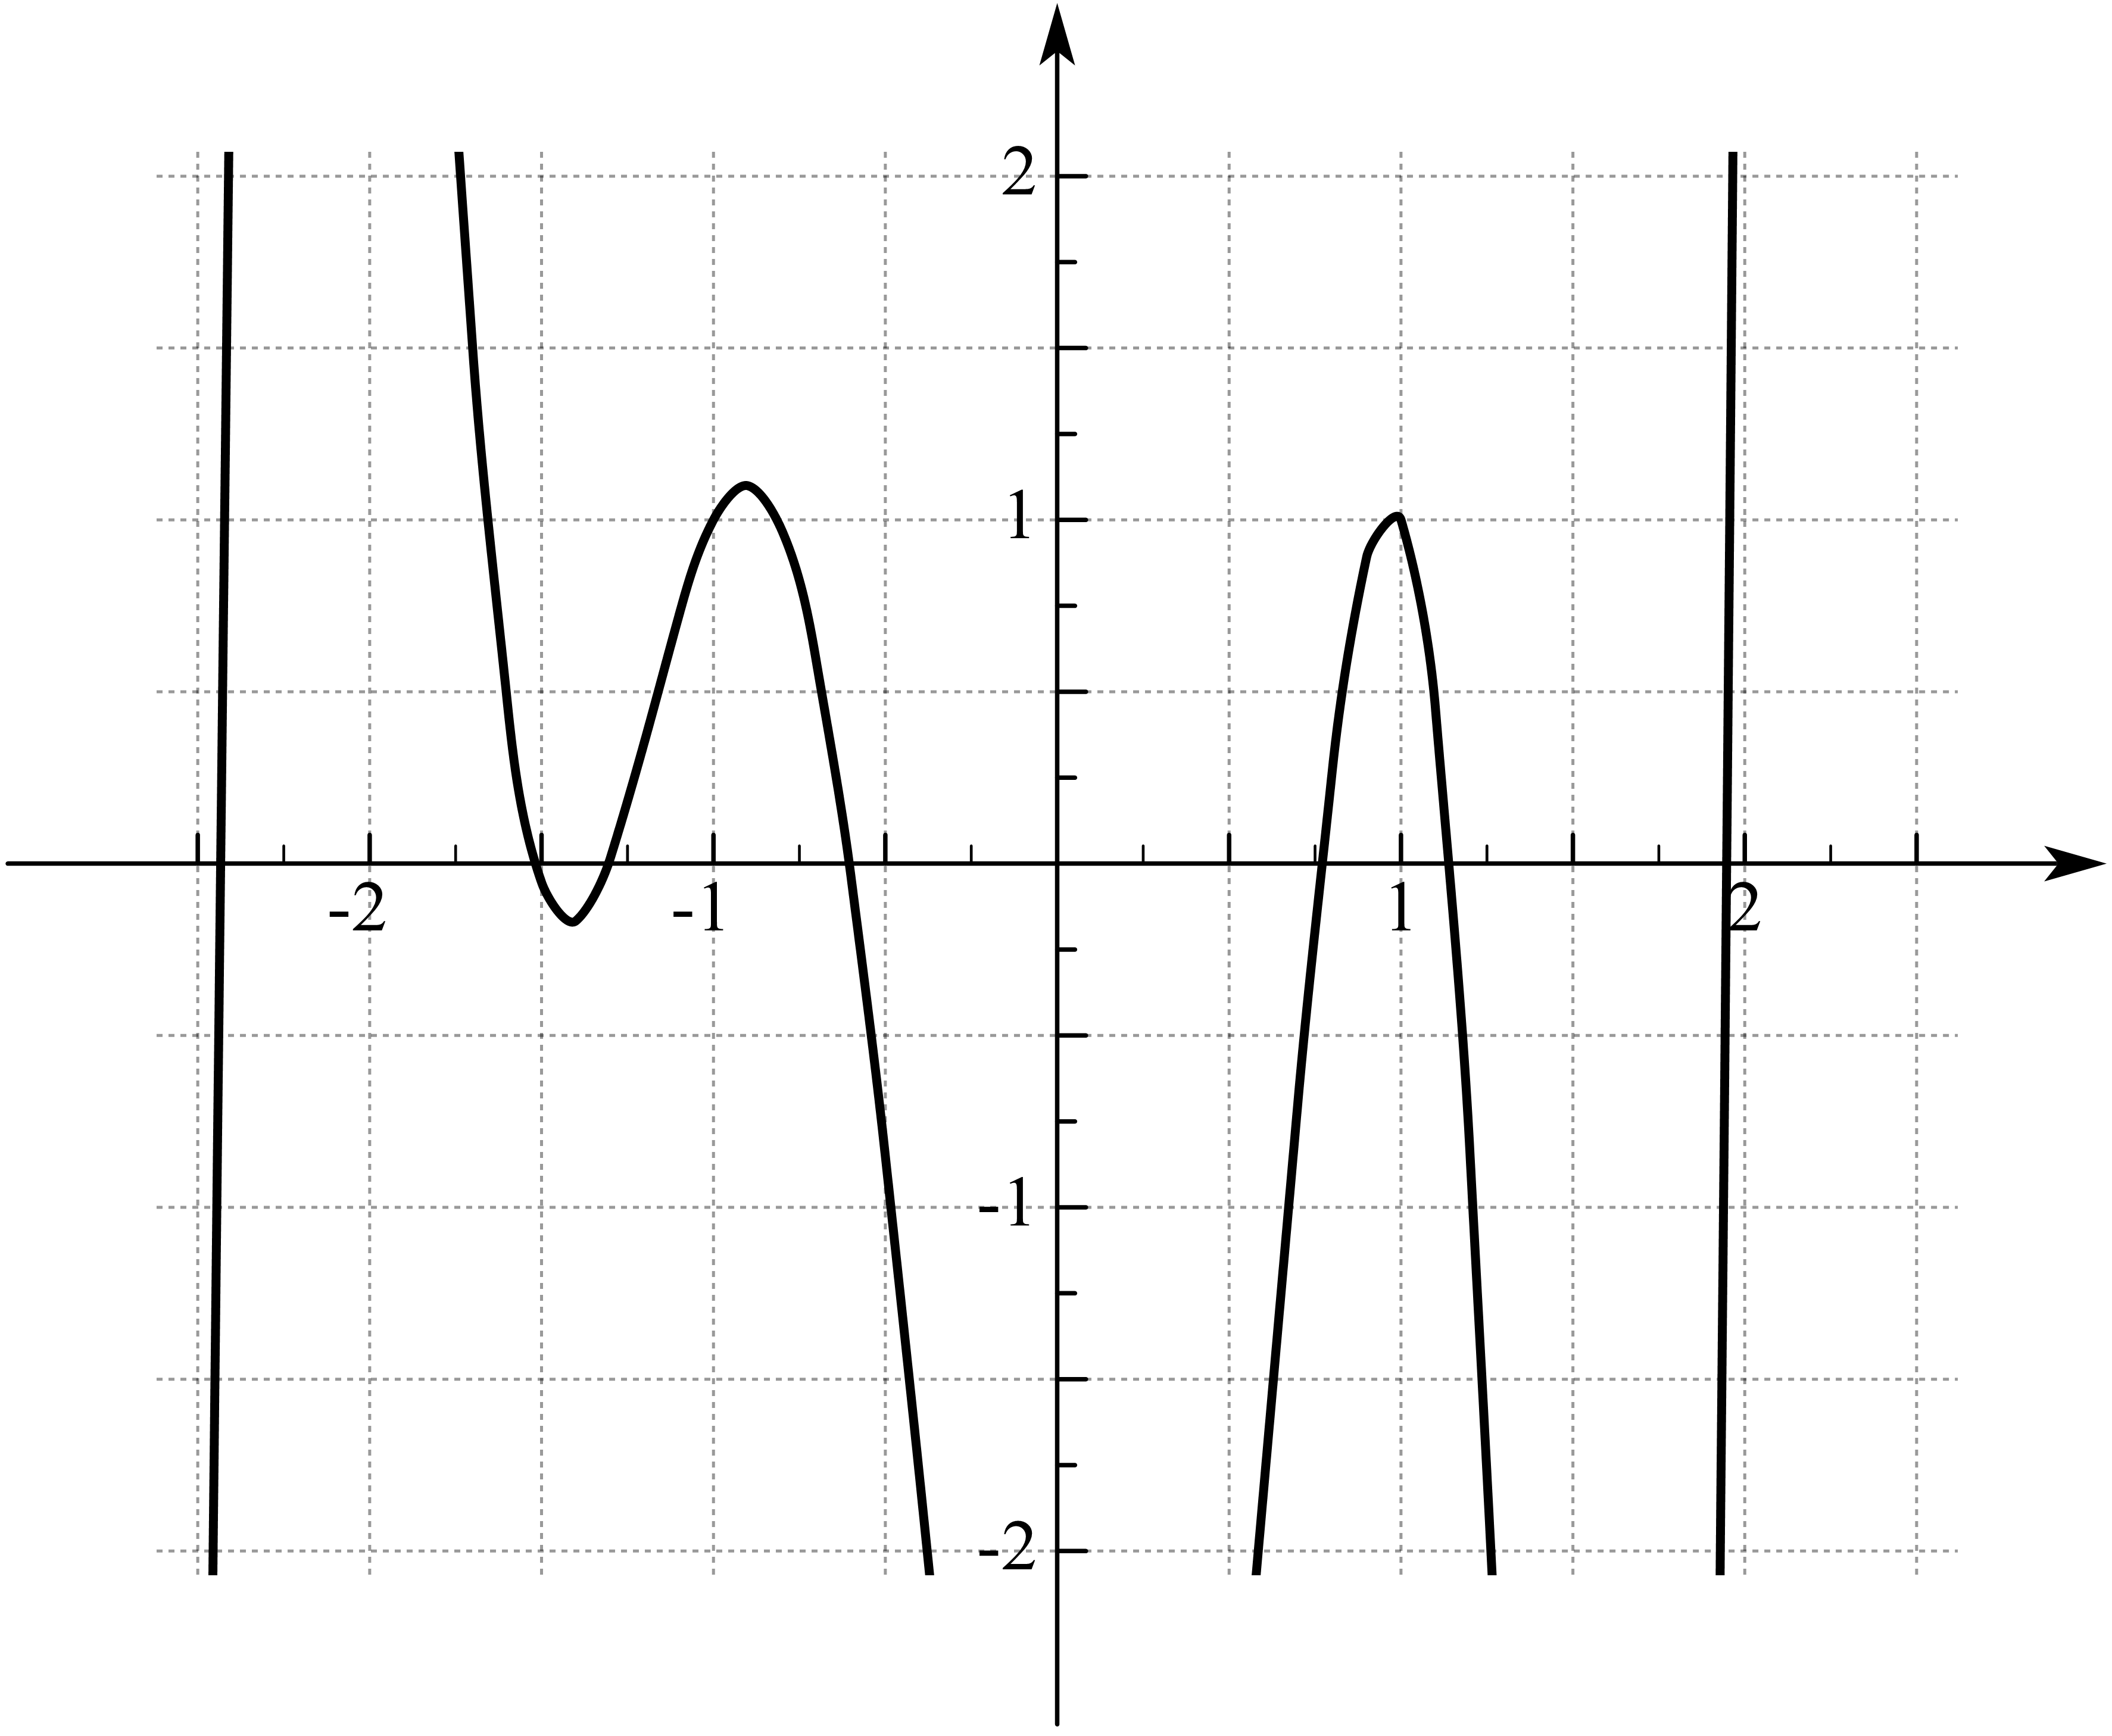
\includegraphics[scale=1]{./structures/exercise_1/phenanthrene/996.png}
		\captionof{figure}{The diagram of function $y=x^7 + 2x^6 - 6x^5 - 11x^4 + 9x^3 +15x^2 -4x -5$ in range $[-2.5,2.5]$.}\label{fig:poly_b1}
		\end{center}
						
		There are also seven roots,
		\begin{center}
		\begin{tabular}{llll}
			$x_8 \approx -2.43476$, & $x_9 \approx -1.51627$, & $x_{10} \approx -1.30580$, & $x_{11} \approx -0.605225 $, \\
			$x_{12} \approx 0.769052$, & $x_{13} \approx 1.14238$, & $x_{14} \approx 1.95063$. &
		\end{tabular}
		\end{center}
		which equal to	
		\begin{align}
			\varepsilon_8 &\approx \alpha + 2.43476 \beta , \\
			\varepsilon_9 &\approx \alpha + 1.51627 \beta , \\
			\varepsilon_{10} &\approx \alpha + 1.30580 \beta , \\
			\varepsilon_{11} &\approx \alpha + 0.605225 \beta , \\
			\varepsilon_{12} &\approx \alpha - 0.769052 \beta , \\
			\varepsilon_{13} &\approx \alpha - 1.14238 \beta , \\
			\varepsilon_{14} &\approx \alpha - 1.95063 \beta .
		\end{align}
		
		And then, their eigenfunctions can be solved. Intermediate and final results are listed below, too.
		\begin{itemize}
		
		\item $\varepsilon_8 \approx \alpha + 2.43476 \beta$
		
		The original eigenfunction is
		\begin{equation*}
			\Phi_8 = 0.83768 \phi^\prime_8 + 0.60476 \phi^\prime_9 + 0.63476 \phi^\prime_{10} + 0.94073 \phi^\prime_{11} + 1.65569 \phi^\prime_{12} + 1.43479 \phi^\prime_{13} + 1.00000 \phi^\prime_{14}.
		\end{equation*}
		
		The sum of coefficients is
		\begin{equation*}
			\sum_{i} c^2_{8,i} = 8.15527.
		\end{equation*}
		
		The normalized eigenfunction is		
		\begin{align}
			\Phi^\pi_8 &\approx 0.350171 \Phi_8 \notag \\
			&\approx 0.29333 \phi^\prime_8 + 0.21177 \phi^\prime_9 + 0.22228 \phi^\prime_{10} + 0.32942 \phi^\prime_{11} + 0.57978 \phi^\prime_{12}  \notag\\
			&\hspace*{22em} + 0.50242 \phi^\prime_{13} + 0.35017 \phi^\prime_{14} \notag \\
			&\approx 0.20742 \phi_1 + 0.14974 \phi_2 + 0.15717 \phi_3 + 0.23293 \phi_4 + 0.40996 \phi_5  \notag \\
			&\hspace*{4em} +0.40996\phi_6 +0.23293 \phi_7 + 0.15717 \phi_8 +0.14974 \phi_9  +0.20742 \phi_{10} \notag \\
			&\hspace*{4em} +0.35527 \phi_{11} + 0.24761 \phi_{12} + 0.24761 \phi_{13} + 0.35527 \phi_{14} .
		\end{align}
		
		
		\item $\varepsilon_9 \approx \alpha + 1.51627 \beta$
		
		The original eigenfunction is
		\begin{equation*}
			\Phi_9 = 0.04360 \phi^\prime_8 - 0.45017 \phi^\prime_9 -0.72618 \phi^\prime_{10} -0.65091 \phi^\prime_{11} -0.26078 \phi^\prime_{12} + 0.51628 \phi^\prime_{13} + 1.00000 \phi^\prime_{14}.
		\end{equation*}
		
		The sum of coefficients is
		\begin{equation*}
			\sum_{i} c^2_{9,i} = 2.49013.
		\end{equation*}
		
		The normalized eigenfunction is		
		\begin{align}
			\Phi^\pi_9 &\approx 0.633708 \Phi_9 \notag \\
			&\approx 0.02763 \phi^\prime_8 - 0.28528 \phi^\prime_9 -0.46018 \phi^\prime_{10} -0.41249 \phi^\prime_{11} -0.16526 \phi^\prime_{12}  \notag\\
			&\hspace*{22em} + 0.32717 \phi^\prime_{13} + 0.63371 \phi^\prime_{14} \notag \\
			&\approx 0.01954 \phi_1 -0.20172 \phi_2 - 0.32540 \phi_3 -0.29167 \phi_4 -0.11686 \phi_5  \notag \\
			&\hspace*{4em} -0.11686 \phi_6 -0.29167 \phi_7 -0.32540\phi_8 -0.20172 \phi_9  +0.01954 \phi_{10} \notag \\
			&\hspace*{4em} +0.23134 \phi_{11} + 0.44810 \phi_{12} + 0.44810 \phi_{13} + 0.23134 \phi_{14} .
		\end{align}
		
		
		\item $\varepsilon_{10} \approx \alpha + 1.30580 \beta$
		
		The original eigenfunction is
		\begin{equation*}
			\Phi_{10} =  3.45516 \phi^\prime_8 + 4.20593 \phi^\prime_9 + 2.03694  \phi^\prime_{10} -1.54608 \phi^\prime_{11}   -4.05582 \phi^\prime_{12} + 0.30582 \phi^\prime_{13} +1.00000 \phi^\prime_{14}.
		\end{equation*}
		
		The sum of coefficients is
		\begin{equation*}
			\sum_{i} c^2_{10,i} =  53.7106.
		\end{equation*}
		
		The normalized eigenfunction is		
		\begin{align}
			\Phi^\pi_{10} &\approx 0.13645 \Phi_{10} \notag \\
			&\approx 0.47145 \phi^\prime_8 + 0.57389 \phi^\prime_9 + 0.27794 \phi^\prime_{10} -0.21096 \phi^\prime_{11} -0.55341 \phi^\prime_{12}  \notag\\
			&\hspace*{22em} + 0.04173 \phi^\prime_{13} + 0.13644 \phi^\prime_{14} \notag \\
			&\approx 0.33337 \phi_1 + 0.40580 \phi_2 + 0.19653  \phi_3 -0.14917 \phi_4  -0.39132 \phi_5  \notag \\
			&\hspace*{4em}  -0.39132 \phi_6  -0.14917 \phi_7 + 0.19653  \phi_8  + 0.40580 \phi_9  + 0.33337 \phi_{10} \notag \\
			&\hspace*{4em} +0.02951 \phi_{11} +0.09648  \phi_{12}  +0.09648 \phi_{13} + 0.02951 \phi_{14} .
		\end{align}
		
		
		\item $\varepsilon_{11} \approx \alpha + 0.605225 \beta$
		
		The original eigenfunction is
		\begin{equation*}
			\Phi_{11} = 0.81967 \phi^\prime_8 + 0.10131  \phi^\prime_9 - 0.75836  \phi^\prime_{10} -0.56029 \phi^\prime_{11} +0.41926 \phi^\prime_{12} +0.39478 \phi^\prime_{13} - 1.00000  \phi^\prime_{14}.
		\end{equation*}
		
		The sum of coefficients is
		\begin{equation*}
			\sum_{i} c^2_{11,i} =  2.90277.
		\end{equation*}
		
		The normalized eigenfunction is		
		\begin{align}
			\Phi^\pi_{11} &\approx 0.586940 \Phi_{11} \notag \\
			&\approx  0.48110 \phi^\prime_8 + 0.05946 \phi^\prime_9 -0.44511 \phi^\prime_{10} -0.32885 \phi^\prime_{11} + 0.24608  \phi^\prime_{12}  \notag\\
			&\hspace*{22em} +0.23171 \phi^\prime_{13} -0.58694 \phi^\prime_{14} \notag \\
			&\approx 0.34019 \phi_1 -0.04205 \phi_2  -0.31474 \phi_3  +0.23253 \phi_4 +0.17400  \phi_5  \notag \\
			&\hspace*{4em} +0.17400  \phi_6  +0.23253  \phi_7 -0.31474 \phi_8  -0.04205 \phi_9 +0.34019 \phi_{10} \notag \\
			&\hspace*{4em} +0.16384 \phi_{11} -0.41503  \phi_{12}   -0.41503 \phi_{13} +0.16384 \phi_{14} .
		\end{align}
		
		
		\item $\varepsilon_{12} \approx \alpha -0.769052 \beta$
		
		The original eigenfunction is
		\begin{equation*}
			\Phi_{12} = 2.70354 \phi^\prime_8 -3.84820 \phi^\prime_9 +0.25592 \phi^\prime_{10} +3.65138 \phi^\prime_{11}  -3.06402 \phi^\prime_{12} +1.76903 \phi^\prime_{13} -1.00000 \phi^\prime_{14}.
		\end{equation*}
		
		The sum of coefficients is
		\begin{equation*}
			\sum_{i} c^2_{12,i} = 49.0335.
		\end{equation*}
		
		The normalized eigenfunction is		
		\begin{align}
			\Phi^\pi_{12} &\approx 0.142808 \Phi_{12} \notag \\
			&\approx 0.38609 \phi^\prime_8 - 0.54955 \phi^\prime_9 + 0.03655 \phi^\prime_{10} + 0.52145 \phi^\prime_{11} - 0.43757  \phi^\prime_{12}  \notag\\
			&\hspace*{22em} +0.25263 \phi^\prime_{13} - 0.14281  \phi^\prime_{14} \notag \\
			&\approx 0.27301 \phi_1 -0.38858  \phi_2  +0.02584 \phi_3 +0.36872 \phi_4 -0.30941  \phi_5  \notag \\
			&\hspace*{4em} -0.30941 \phi_6  +0.36872 \phi_7 +0.02584 \phi_8  -0.38858 \phi_9 +0.27301 \phi_{10} \notag \\
			&\hspace*{4em} +0.17864 \phi_{11} -0.10098  \phi_{12}   -0.10098 \phi_{13}  +0.17864 \phi_{14} .
		\end{align}
		
		
		\item $\varepsilon_{13} \approx \alpha - 1.14238 \beta$
		
		The original eigenfunction is
		\begin{equation*}
			\Phi_{13} =  1.19554 \phi^\prime_8 + 0.77669 \phi^\prime_9 -2.08281  \phi^\prime_{10} + 1.60267 \phi^\prime_{11}   +0.25195 \phi^\prime_{12} -2.14244 \phi^\prime_{13} + 1.00000 \phi^\prime_{14}.
		\end{equation*}
		
		The sum of coefficients is
		\begin{equation*}
			\sum_{i} c^2_{13,i} = 14.5927.
		\end{equation*}
		
		The normalized eigenfunction is		
		\begin{align}
			\Phi^\pi_{13} &\approx  0.261777 \Phi_{13} \notag \\
			&\approx  0.31296 \phi^\prime_8 + 0.20332 \phi^\prime_9  -0.54523 \phi^\prime_{10} +0.41954 \phi^\prime_{11} + 0.06596  \phi^\prime_{12}  \notag\\
			&\hspace*{22em} -0.56084 \phi^\prime_{13} + 0.26178  \phi^\prime_{14} \notag \\
			&\approx  0.22130 \phi_1 +0.14377 \phi_2 -0.38554  \phi_3 +0.29666 \phi_4 + 0.04664  \phi_5  \notag \\
			&\hspace*{4em} + 0.04664  \phi_6  +0.29666 \phi_7 -0.38554  \phi_8  +0.14377 \phi_9 + 0.22130 \phi_{10} \notag \\
			&\hspace*{4em}  -0.39658 \phi_{11} +0.18510 \phi_{12}  +0.18510 \phi_{13} -0.39658 \phi_{14} .
		\end{align}
		
		
		\item $\varepsilon_{14} \approx \alpha - 1.95063 \beta$
		
		The original eigenfunction is
		\begin{equation*}
			\Phi_{14} =  2.99111 \phi^\prime_8 -2.88404 \phi^\prime_9 + 2.63460 \phi^\prime_{10} -2.25508 \phi^\prime_{11}   + 1.76423 \phi^\prime_{12} - 2.95050  \phi^\prime_{13} + 1.00000 \phi^\prime_{14}.
		\end{equation*}
		
		The sum of coefficients is
		\begin{equation*}
			\sum_{i} c^2_{14,i} = 42.1088
		\end{equation*}
		
		The normalized eigenfunction is		
		\begin{align}
			\Phi^\pi_{14} &\approx 0.154104 \Phi_{14} \notag \\
			&\approx 0.46094 \phi^\prime_8 -0.44444 \phi^\prime_9  + 0.40600 \phi^\prime_{10} -0.34752 \phi^\prime_{11} + 0.27187 \phi^\prime_{12}  \notag\\
			&\hspace*{22em} -0.45468 \phi^\prime_{13} + 0.15410 \phi^\prime_{14} \notag \\
			&\approx 0.32594 \phi_1 -0.31427 \phi_2  + 0.28709 \phi_3 -0.24573 \phi_4 +0.19224 \phi_5  \notag \\
			&\hspace*{4em}  +0.19224 \phi_6  -0.24573 \phi_7 + 0.28709 \phi_8  -0.31427 \phi_9   + 0.32594 \phi_{10} \notag \\
			&\hspace*{4em} -0.32151 \phi_{11} + 0.10897 \phi_{12}  + 0.10897 \phi_{13} -0.32151 \phi_{14} .
		\end{align}
		
		\end{itemize}
		
		In conclusion, for the irreducible representation $\Gamma^{B_1}$, relevant results are listed below.
		\begin{center}
		\setlength{\abovecaptionskip}{0em}
		\captionof{table}{The H{\"u}ckel MOs in the irreducible representation $\Gamma^{B_1}$ of phenanthrene.}
		\begin{tabular}{ccccccccc}\hline
		order & eigenvalue & \multicolumn{7}{c}{eigenfunction} \\ \hline
	\multirow{4}*{1}	&	\multirow{4}*{$\alpha+2.435\beta$}	& $c_1$ & $c_2$ & $c_3$ & $c_4$ & $c_5$ & $c_6$ & $c_7$\\\cline{3-9}
& & 0.2074 & 0.1497 & 0.1572 & 0.2329 & 0.4100 & 0.4100 & 0.2329 \\ \cline{3-9}
& & $c_8$ & $c_9$ & $c_{10}$ & $c_{11}$ & $c_{12}$ & $c_{13}$ & $c_{14}$\\\cline{3-9}
& & 0.1572 & 0.1497 & 0.2074 & 0.3553 & 0.2476 & 0.2476 & 0.3553 \\ \hline
	\multirow{4}*{2}	&	\multirow{4}*{$\alpha+1.516\beta$}	& $c_1$ & $c_2$ & $c_3$ & $c_4$ & $c_5$ & $c_6$ & $c_7$\\\cline{3-9}
& & 0.0195 & -0.2017 & -0.3254 & -0.2917 & -0.1169 & -0.1169 & -0.2917 \\ \cline{3-9}
& & $c_8$ & $c_9$ & $c_{10}$ & $c_{11}$ & $c_{12}$ & $c_{13}$ & $c_{14}$\\\cline{3-9}
& & -0.3254 & -0.2017 & 0.0195 & 0.2313 & 0.4481 & 0.4481 & 0.2313 \\ \hline
	\multirow{4}*{3}	&	\multirow{4}*{$\alpha+1.306\beta$}	& $c_1$ & $c_2$ & $c_3$ & $c_4$ & $c_5$ & $c_6$ & $c_7$\\\cline{3-9}
& & 0.3334 & 0.4058 & 0.1965 & -0.1492 & -0.3913 & -0.3913 & -0.1492 \\ \cline{3-9}
& & $c_8$ & $c_9$ & $c_{10}$ & $c_{11}$ & $c_{12}$ & $c_{13}$ & $c_{14}$\\\cline{3-9}
& & 0.1965 & 0.4058 & 0.3334 & 0.0295 & 0.0965 & 0.0965 & 0.0295 \\ \hline
\multirow{4}*{4}	&	\multirow{4}*{$\alpha+0.605\beta$}	& $c_1$ & $c_2$ & $c_3$ & $c_4$ & $c_5$ & $c_6$ & $c_7$\\\cline{3-9}
& & 0.3402 & -0.0420 & -0.3147 & 0.2325 & 0.1740 & 0.1740 & 0.2325 \\ \cline{3-9}
& & $c_8$ & $c_9$ & $c_{10}$ & $c_{11}$ & $c_{12}$ & $c_{13}$ & $c_{14}$\\\cline{3-9}
& & -0.3147 & -0.0420 & 0.3402 & 0.1638 & -0.4150 & -0.4150 & 0.1638 \\ \hline
\multirow{4}*{5}	&	\multirow{4}*{$\alpha-0.769\beta$}	& $c_1$ & $c_2$ & $c_3$ & $c_4$ & $c_5$ & $c_6$ & $c_7$\\\cline{3-9}
& & 0.2730 & -0.3886 & 0.0258 & 0.3687 & -0.3094 & -0.3094 & 0.3687 \\ \cline{3-9}
& & $c_8$ & $c_9$ & $c_{10}$ & $c_{11}$ & $c_{12}$ & $c_{13}$ & $c_{14}$\\\cline{3-9}
& & 0.0258 & -0.3886 & 0.2730 & 0.1786 & -0.1010 & -0.1010 & 0.1786 \\ \hline
\multirow{4}*{6}	&	\multirow{4}*{$\alpha-1.142\beta$}	& $c_1$ & $c_2$ & $c_3$ & $c_4$ & $c_5$ & $c_6$ & $c_7$\\\cline{3-9}
& & 0.2213 & 0.1438 & -0.3855 & 0.2967 & 0.0466 & 0.0466 & 0.2967 \\ \cline{3-9}
& & $c_8$ & $c_9$ & $c_{10}$ & $c_{11}$ & $c_{12}$ & $c_{13}$ & $c_{14}$\\\cline{3-9}
& & -0.3855 & 0.1438 & 0.2213 & -0.3966 & 0.1851 & 0.1851 & -0.3966 \\ \hline
\multirow{4}*{7}	&	\multirow{4}*{$\alpha-1.951\beta$}	& $c_1$ & $c_2$ & $c_3$ & $c_4$ & $c_5$ & $c_6$ & $c_7$\\\cline{3-9}
& & 0.3259 & -0.3143 & 0.2871 & -0.2457 & 0.1922 & 0.1922 & -0.2457 \\ \cline{3-9}
& & $c_8$ & $c_9$ & $c_{10}$ & $c_{11}$ & $c_{12}$ & $c_{13}$ & $c_{14}$\\\cline{3-9}
& & 0.2871 & -0.3143 & 0.3259 & -0.3215 & 0.1090 & 0.1090 & -0.3215 \\ \hline
		\end{tabular}
		\end{center}
		
		Now, we have obtained all results, which are shown in \Tableref{tab:result_6}
		\begin{center}
		\captionof{table}{The occupied H{\"u}ckel MOs in all irreducible representations of phenanthrene.}\label{tab:result_6}
		\begin{longtable}{cccccccccc}\hline
		order 	& orbital energy & irrep & \multicolumn{7}{c}{eigenfunction} \\ \hline
		\multirow{4}*{1}	&	\multirow{4}*{$\alpha+2.435\beta$}	&	\multirow{4}*{$B_1$} & $c_1$ & $c_2$ & $c_3$ & $c_4$ & $c_5$ & $c_6$ & $c_7$\\\cline{4-10}
& & & 0.2074 & 0.1497 & 0.1572 & 0.2329 & 0.4100 & 0.4100 & 0.2329 \\ \cline{4-10}
& & & $c_8$ & $c_9$ & $c_{10}$ & $c_{11}$ & $c_{12}$ & $c_{13}$ & $c_{14}$\\\cline{4-10}
& & & 0.1572 & 0.1497 & 0.2074 & 0.3553 & 0.2476 & 0.2476 & 0.3553 \\ \hline
		\multirow{4}*{2}	&	\multirow{4}*{$\alpha+1.951\beta$}	&   \multirow{4}*{$A_2$}&$c_1$ & $c_2$ & $c_3$ & $c_4$ & $c_5$ & $c_6$ & $c_7$\\\cline{4-10}
& & &0.3259 & 0.3143 & 0.2871 & 0.2457 & 0.1922 & -0.1922 & -0.2457 \\ \cline{4-10}
& & &$c_8$ & $c_9$ & $c_{10}$ & $c_{11}$ & $c_{12}$ & $c_{13}$ & $c_{14}$\\\cline{4-10}
& & &-0.2871 & -0.3143 & -0.3259 & -0.3215 & -0.1090 & 0.1090 & 0.3215 \\ \hline
		\multirow{4}*{3}	&	\multirow{4}*{$\alpha+1.516\beta$}	&  \multirow{4}*{$B_1$} & $c_1$ & $c_2$ & $c_3$ & $c_4$ & $c_5$ & $c_6$ & $c_7$\\\cline{4-10}
& & & 0.0195 & -0.2017 & -0.3254 & -0.2917 & -0.1169 & -0.1169 & -0.2917 \\ \cline{4-10}
& & & $c_8$ & $c_9$ & $c_{10}$ & $c_{11}$ & $c_{12}$ & $c_{13}$ & $c_{14}$\\\cline{4-10}
& & & -0.3254 & -0.2017 & 0.0195 & 0.2313 & 0.4481 & 0.4481 & 0.2313 \\ \hline
		\multirow{4}*{4}	&	\multirow{4}*{$\alpha+1.306\beta$}	&\multirow{4}*{$B_1$} & $c_1$ & $c_2$ & $c_3$ & $c_4$ & $c_5$ & $c_6$ & $c_7$\\\cline{4-10}
& & & 0.3334 & 0.4058 & 0.1965 & -0.1492 & -0.3913 & -0.3913 & -0.1492 \\ \cline{4-10}
& & & $c_8$ & $c_9$ & $c_{10}$ & $c_{11}$ & $c_{12}$ & $c_{13}$ & $c_{14}$\\\cline{4-10}
& & & 0.1965 & 0.4058 & 0.3334 & 0.0295 & 0.0965 & 0.0965 & 0.0295 \\ \hline
		\multirow{4}*{5}	&	\multirow{4}*{$\alpha+1.142\beta$}	&   \multirow{4}*{$A_2$} & $c_1$ & $c_2$ & $c_3$ & $c_4$ & $c_5$ & $c_6$ & $c_7$\\\cline{4-10}
& & &0.2213 & -0.1438 & -0.3855 & -0.2967 & 0.0466 & -0.0466 & 0.2967 \\ \cline{4-10}
& & &$c_8$ & $c_9$ & $c_{10}$ & $c_{11}$ & $c_{12}$ & $c_{13}$ & $c_{14}$\\\cline{4-10}
& & &0.3855 & 0.1438 & -0.2213 & -0.3966 & -0.1851 & 0.1851 & 0.3966 \\ \hline
		\multirow{4}*{6}	&	\multirow{4}*{$\alpha+0.769\beta$}	& \multirow{4}*{$A_2$}&  $c_1$ & $c_2$ & $c_3$ & $c_4$ & $c_5$ & $c_6$ & $c_7$\\\cline{4-10}
& & &0.2730 & 0.3886 & 0.0258 & -0.3687 & -0.3094 & 0.3094 & 0.3687 \\ \cline{4-10}
& & &$c_8$ & $c_9$ & $c_{10}$ & $c_{11}$ & $c_{12}$ & $c_{13}$ & $c_{14}$\\\cline{4-10}
& & & -0.0258 & -0.3886 & -0.2730 & 0.1786 & 0.1010 & -0.1010 & -0.1786 \\ \hline
		\multirow{4}*{7}	&	\multirow{4}*{$\alpha+0.605\beta$}	&\multirow{4}*{$B_1$} & $c_1$ & $c_2$ & $c_3$ & $c_4$ & $c_5$ & $c_6$ & $c_7$\\\cline{4-10}
& & &0.3402 & -0.0420 & -0.3147 & 0.2325 & 0.1740 & 0.1740 & 0.2325 \\ \cline{4-10}
& & &$c_8$ & $c_9$ & $c_{10}$ & $c_{11}$ & $c_{12}$ & $c_{13}$ & $c_{14}$\\\cline{4-10}
& & &-0.3147 & -0.0420 & 0.3402 & 0.1638 & -0.4150 & -0.4150 & 0.1638 \\ \hline
		\multirow{4}*{8}	&	\multirow{4}*{$\alpha-0.605\beta$} & \multirow{4}*{$A_2$}	& $c_1$ & $c_2$ & $c_3$ & $c_4$ & $c_5$ & $c_6$ & $c_7$\\\cline{4-10}
& & & 0.3402 & -0.0420 & -0.3147 & 0.2325 & 0.1740 & -0.1740 & -0.2325 \\ \cline{4-10}
& & &$c_8$ & $c_9$ & $c_{10}$ & $c_{11}$ & $c_{12}$ & $c_{13}$ & $c_{14}$\\\cline{4-10}
& & & 0.3147 & 0.0420 & -0.3402 & 0.1638 & 0.4150 & -0.4150 & -0.1638 \\ \hline
		\multirow{4}*{9}	&	\multirow{4}*{$\alpha-0.769\beta$}	&\multirow{4}*{$B_1$} & $c_1$ & $c_2$ & $c_3$ & $c_4$ & $c_5$ & $c_6$ & $c_7$\\\cline{4-10}
& & & 0.2730 & -0.3886 & 0.0258 & 0.3687 & -0.3094 & -0.3094 & 0.3687 \\ \cline{4-10}
& & & $c_8$ & $c_9$ & $c_{10}$ & $c_{11}$ & $c_{12}$ & $c_{13}$ & $c_{14}$\\\cline{4-10}
& & & 0.0258 & -0.3886 & 0.2730 & 0.1786 & -0.1010 & -0.1010 & 0.1786 \\ \hline
		\multirow{4}*{10}	&	\multirow{4}*{$\alpha-1.142\beta$} &	\multirow{4}*{$B_1$} & $c_1$ & $c_2$ & $c_3$ & $c_4$ & $c_5$ & $c_6$ & $c_7$\\\cline{4-10}
& & & 0.2213 & 0.1438 & -0.3855 & 0.2967 & 0.0466 & 0.0466 & 0.2967 \\ \cline{4-10}
& & & $c_8$ & $c_9$ & $c_{10}$ & $c_{11}$ & $c_{12}$ & $c_{13}$ & $c_{14}$\\\cline{4-10}
& & & -0.3855 & 0.1438 & 0.2213 & -0.3966 & 0.1851 & 0.1851 & -0.3966 \\ \hline
		\multirow{4}*{11}	&	\multirow{4}*{$\alpha-1.306\beta$} & \multirow{4}*{$A_2$} & $c_1$ & $c_2$ & $c_3$ & $c_4$ & $c_5$ & $c_6$ & $c_7$\\\cline{4-10}
& & & 0.3334 & -0.4058 & 0.1965 & 0.1492 & -0.3913 & 0.3913 & -0.1492 \\ \cline{4-10}
& & & $c_8$ & $c_9$ & $c_{10}$ & $c_{11}$ & $c_{12}$ & $c_{13}$ & $c_{14}$\\\cline{4-10}
& & & -0.1965 & 0.4058 & -0.3334 & 0.0295 & -0.0965 & 0.0965 & -0.0295 \\ \hline
		\multirow{4}*{12}	&	\multirow{4}*{$\alpha-1.516\beta$}	&\multirow{4}*{$A_2$} & $c_1$ & $c_2$ & $c_3$ & $c_4$ & $c_5$ & $c_6$ & $c_7$\\\cline{4-10}
& & & 0.0195 & 0.2017 & -0.3254 & 0.2917 & -0.1169 & 0.1169 & -0.2917 \\ \cline{4-10}
& & & $c_8$ & $c_9$ & $c_{10}$ & $c_{11}$ & $c_{12}$ & $c_{13}$ & $c_{14}$\\\cline{4-10}
& & & 0.3254 & -0.2017 & -0.0195 & 0.2313 & -0.4481 & 0.4481 & -0.2313 \\ \hline
		\multirow{4}*{13}	&	\multirow{4}*{$\alpha-1.951\beta$}	& \multirow{4}*{$B_1$} & $c_1$ & $c_2$ & $c_3$ & $c_4$ & $c_5$ & $c_6$ & $c_7$\\\cline{4-10}
& & & 0.3259 & -0.3143 & 0.2871 & -0.2457 & 0.1922 & 0.1922 & -0.2457 \\ \cline{4-10}
& & & $c_8$ & $c_9$ & $c_{10}$ & $c_{11}$ & $c_{12}$ & $c_{13}$ & $c_{14}$\\\cline{4-10}
& & & 0.2871 & -0.3143 & 0.3259 & -0.3215 & 0.1090 & 0.1090 & -0.3215 \\ \hline
		\multirow{4}*{14}	&	\multirow{4}*{$\alpha-2.435\beta$}&\multirow{4}*{$A_2$}	& $c_1$ & $c_2$ & $c_3$ & $c_4$ & $c_5$ & $c_6$ & $c_7$\\\cline{4-10}
& & & 0.2074 & -0.1497 & 0.1572 & -0.2329 & 0.4100 & -0.4100 & 0.2329 \\ \cline{4-10}
& & & $c_8$ & $c_9$ & $c_{10}$ & $c_{11}$ & $c_{12}$ & $c_{13}$ & $c_{14}$\\\cline{4-10}
& & & -0.1572 & 0.1497 & -0.2074 & 0.3553 & -0.2476 & 0.2476 & -0.3553 \\ \hline
		\end{longtable}
		\vspace*{-2em}
		\end{center}		
		
		Besides, their phase diagrams have been painted in \Figref{fig:phase_diagram_6}.
		
		\begin{center}
		\begin{tabular}{cccc}
			\begin{minipage}[t]{0.21\linewidth}
			\centering
			\setlength{\abovecaptionskip}{0.5em}
			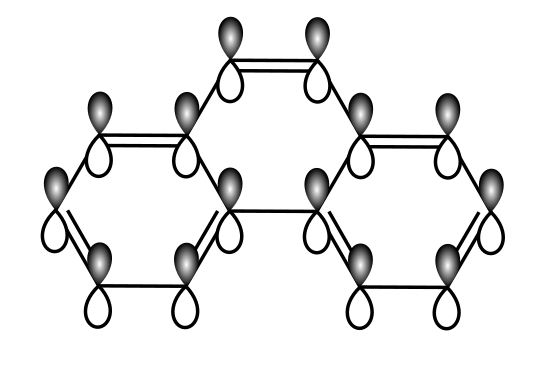
\includegraphics[scale=0.66]{./structures/exercise_1/phenanthrene/8.png}
			\captionof*{figure}{$\varepsilon = \alpha + 2.435\beta$}
			\end{minipage} & 
			\begin{minipage}[t]{0.21\linewidth}
			\setlength{\abovecaptionskip}{0.5em}
			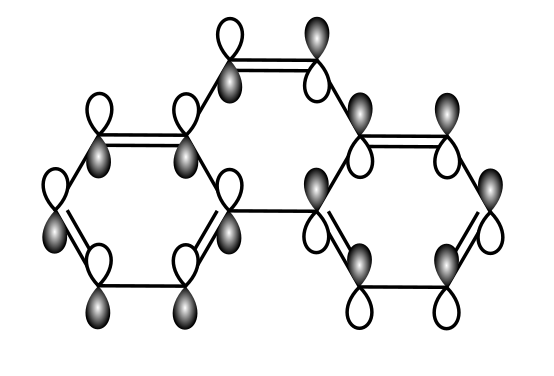
\includegraphics[scale=0.66]{./structures/exercise_1/phenanthrene/1.png}
			\captionof*{figure}{$\varepsilon = \alpha + 1.951\beta$}
			\end{minipage} &
			\begin{minipage}[t]{0.21\linewidth}
			\centering
			\setlength{\abovecaptionskip}{0.5em}
			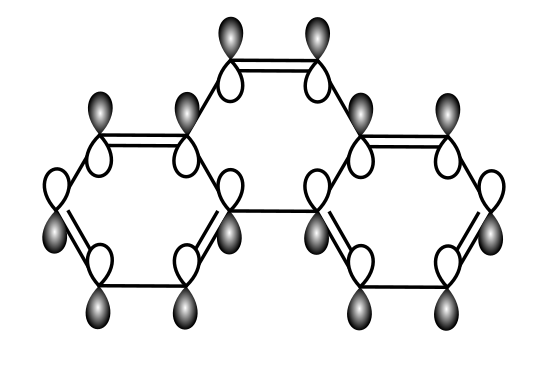
\includegraphics[scale=0.66]{./structures/exercise_1/phenanthrene/9.png}
			\captionof*{figure}{$\varepsilon = \alpha + 1.516\beta$}
			\end{minipage} &
			\begin{minipage}[t]{0.21\linewidth}
			\setlength{\abovecaptionskip}{0.5em}
			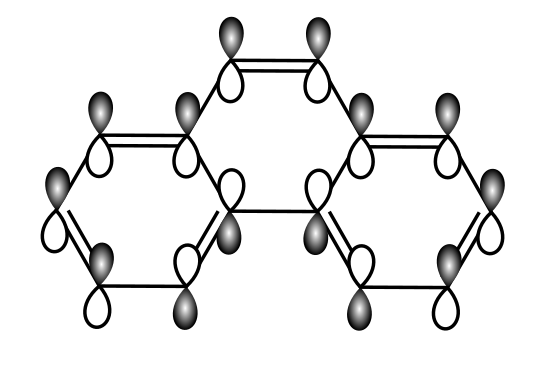
\includegraphics[scale=0.66]{./structures/exercise_1/phenanthrene/10.png}
			\captionof*{figure}{$\varepsilon = \alpha + 1.306\beta$}
			\end{minipage} \\
			\begin{minipage}[t]{0.21\linewidth}
			\centering
			\setlength{\abovecaptionskip}{0.5em}
			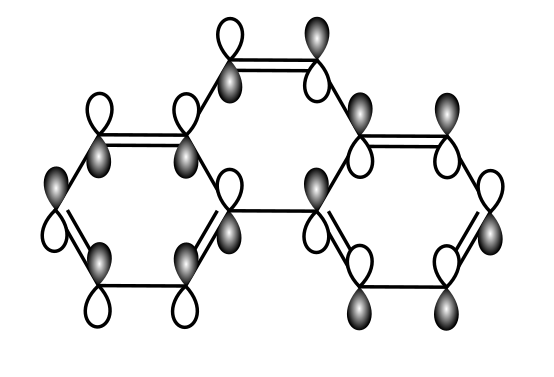
\includegraphics[scale=0.66]{./structures/exercise_1/phenanthrene/2.png}
			\captionof*{figure}{$\varepsilon = \alpha + 1.142\beta$}
			\end{minipage} & 
			\begin{minipage}[t]{0.21\linewidth}
			\setlength{\abovecaptionskip}{0.5em}
			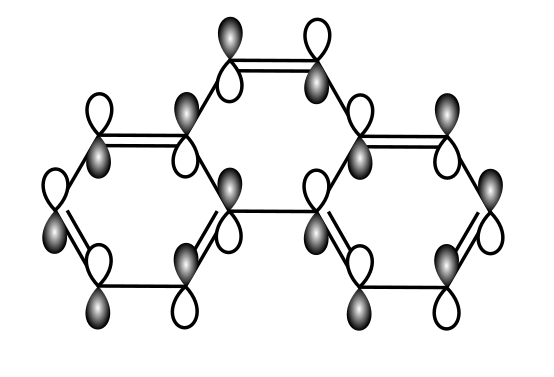
\includegraphics[scale=0.66]{./structures/exercise_1/phenanthrene/3.png}
			\captionof*{figure}{$\varepsilon = \alpha + 0.769\beta$}
			\end{minipage} &
			\begin{minipage}[t]{0.21\linewidth}
			\centering
			\setlength{\abovecaptionskip}{0.5em}
			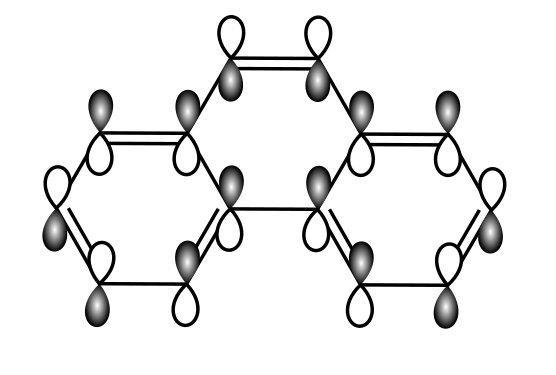
\includegraphics[scale=0.66]{./structures/exercise_1/phenanthrene/11.png}
			\captionof*{figure}{$\varepsilon = \alpha + 0.605\beta$}
			\end{minipage} &
			\begin{minipage}[t]{0.21\linewidth}
			\setlength{\abovecaptionskip}{0.5em}
			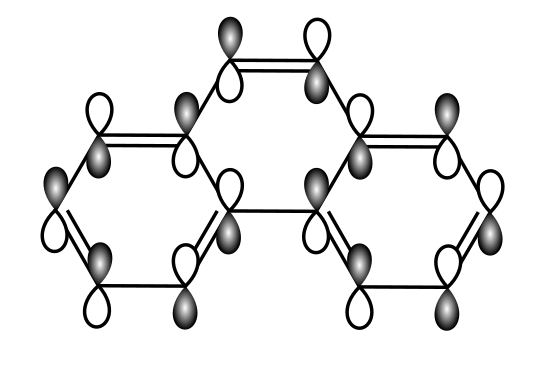
\includegraphics[scale=0.66]{./structures/exercise_1/phenanthrene/4.png}
			\captionof*{figure}{$\varepsilon = \alpha - 0.605\beta$}
			\end{minipage} \\
			\begin{minipage}[t]{0.21\linewidth}
			\centering
			\setlength{\abovecaptionskip}{0.5em}
			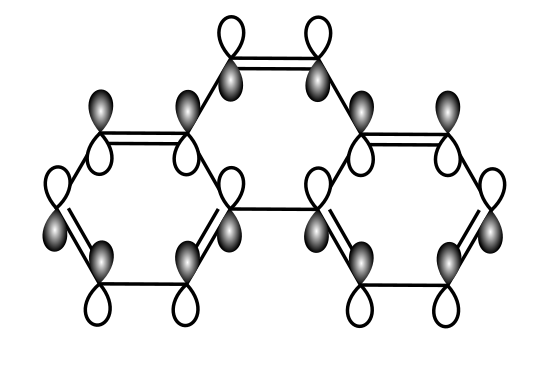
\includegraphics[scale=0.66]{./structures/exercise_1/phenanthrene/12.png}
			\captionof*{figure}{$\varepsilon = \alpha - 0.769\beta$}
			\end{minipage} & 
			\begin{minipage}[t]{0.21\linewidth}
			\setlength{\abovecaptionskip}{0.5em}
			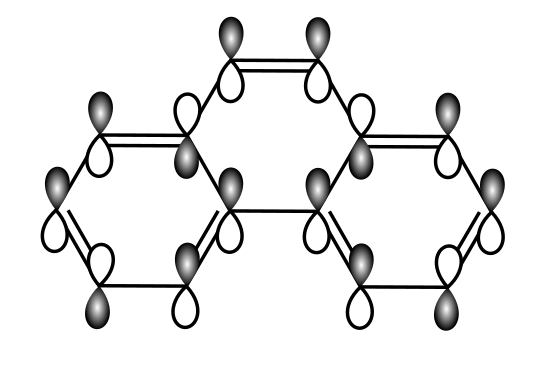
\includegraphics[scale=0.66]{./structures/exercise_1/phenanthrene/13.png}
			\captionof*{figure}{$\varepsilon = \alpha - 1.142\beta$}
			\end{minipage} &
			\begin{minipage}[t]{0.21\linewidth}
			\centering
			\setlength{\abovecaptionskip}{0.5em}
			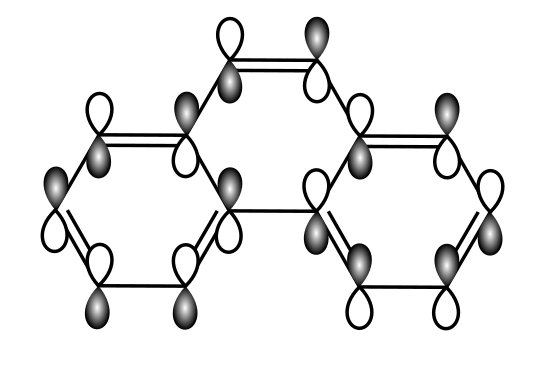
\includegraphics[scale=0.66]{./structures/exercise_1/phenanthrene/5.png}
			\captionof*{figure}{$\varepsilon = \alpha - 1.306\beta$}
			\end{minipage} &
			\begin{minipage}[t]{0.21\linewidth}
			\setlength{\abovecaptionskip}{0.5em}
			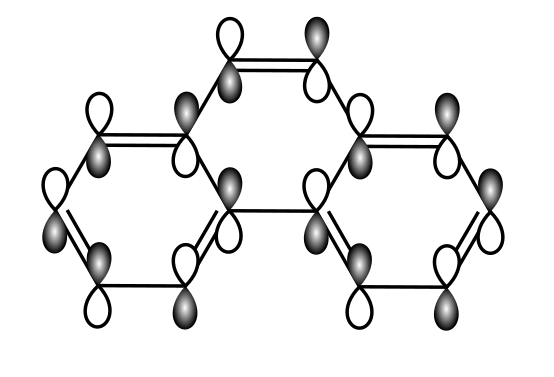
\includegraphics[scale=0.66]{./structures/exercise_1/phenanthrene/6.png}
			\captionof*{figure}{$\varepsilon = \alpha - 1.516\beta$}
			\end{minipage} \\
			\begin{minipage}[t]{0.21\linewidth}
			\centering
			\setlength{\abovecaptionskip}{0.5em}
			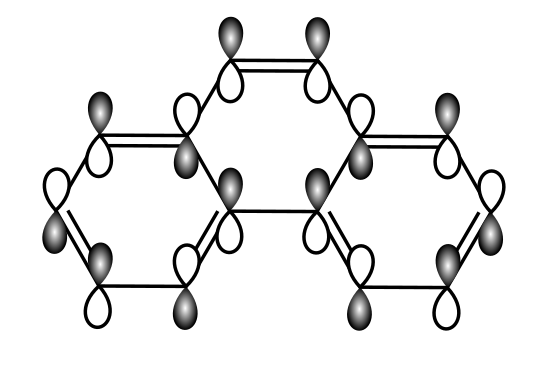
\includegraphics[scale=0.66]{./structures/exercise_1/phenanthrene/14.png}
			\captionof*{figure}{$\varepsilon = \alpha - 1.951\beta$}
			\end{minipage} & 
			\begin{minipage}[t]{0.21\linewidth}
			\setlength{\abovecaptionskip}{0.5em}
			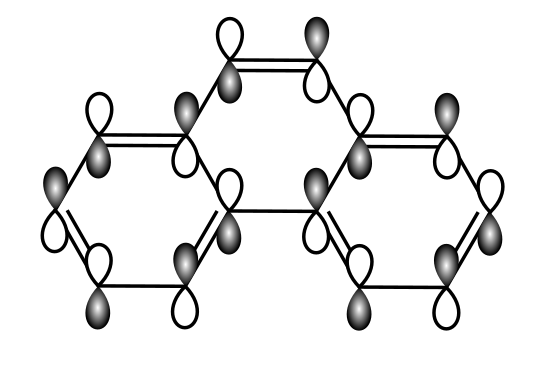
\includegraphics[scale=0.66]{./structures/exercise_1/phenanthrene/7.png}
			\captionof*{figure}{$\varepsilon = \alpha - 2.435\beta$}
			\end{minipage} &
			\begin{minipage}[t]{0.21\linewidth}
			\end{minipage} &
			\begin{minipage}[t]{0.21\linewidth}
			\end{minipage} \\
		\end{tabular}				
		\captionof{figure}{Phase diagrams of these H{\"u}ckel MOs of phenanthrene. Black bubbles mean plus phase while white ones mean minus phase. The color is used just for determining relative phase.}\label{fig:phase_diagram_6}
		\end{center}
		
		In the end, we conclude that for phenanthrene, its ground state $\pi$-electron configuration is $(1b_1)^2 (1a_2)^2 (2b_1)^2 (3b_1)^2 (2a_2)^2 (3a_2)^2 (4b_1)^2$ and its delocalization energy is $2 \times 2.435 \beta + 2 \times 1.951 \beta + 2 \times 1.516 \beta + 2 \times 1.306 \beta + 2 \times 1.142 \beta + 2 \times 0.769 \beta + 2 \times 0.605 \beta - 14 \times 1.000 \beta = 5.448 \beta$, much larger than the sum of that of {\it trans}-1,3-butadiene ($0.472\beta$) and two benzenes ($2.000\beta \times 2$). 
		
		\begin{center}
		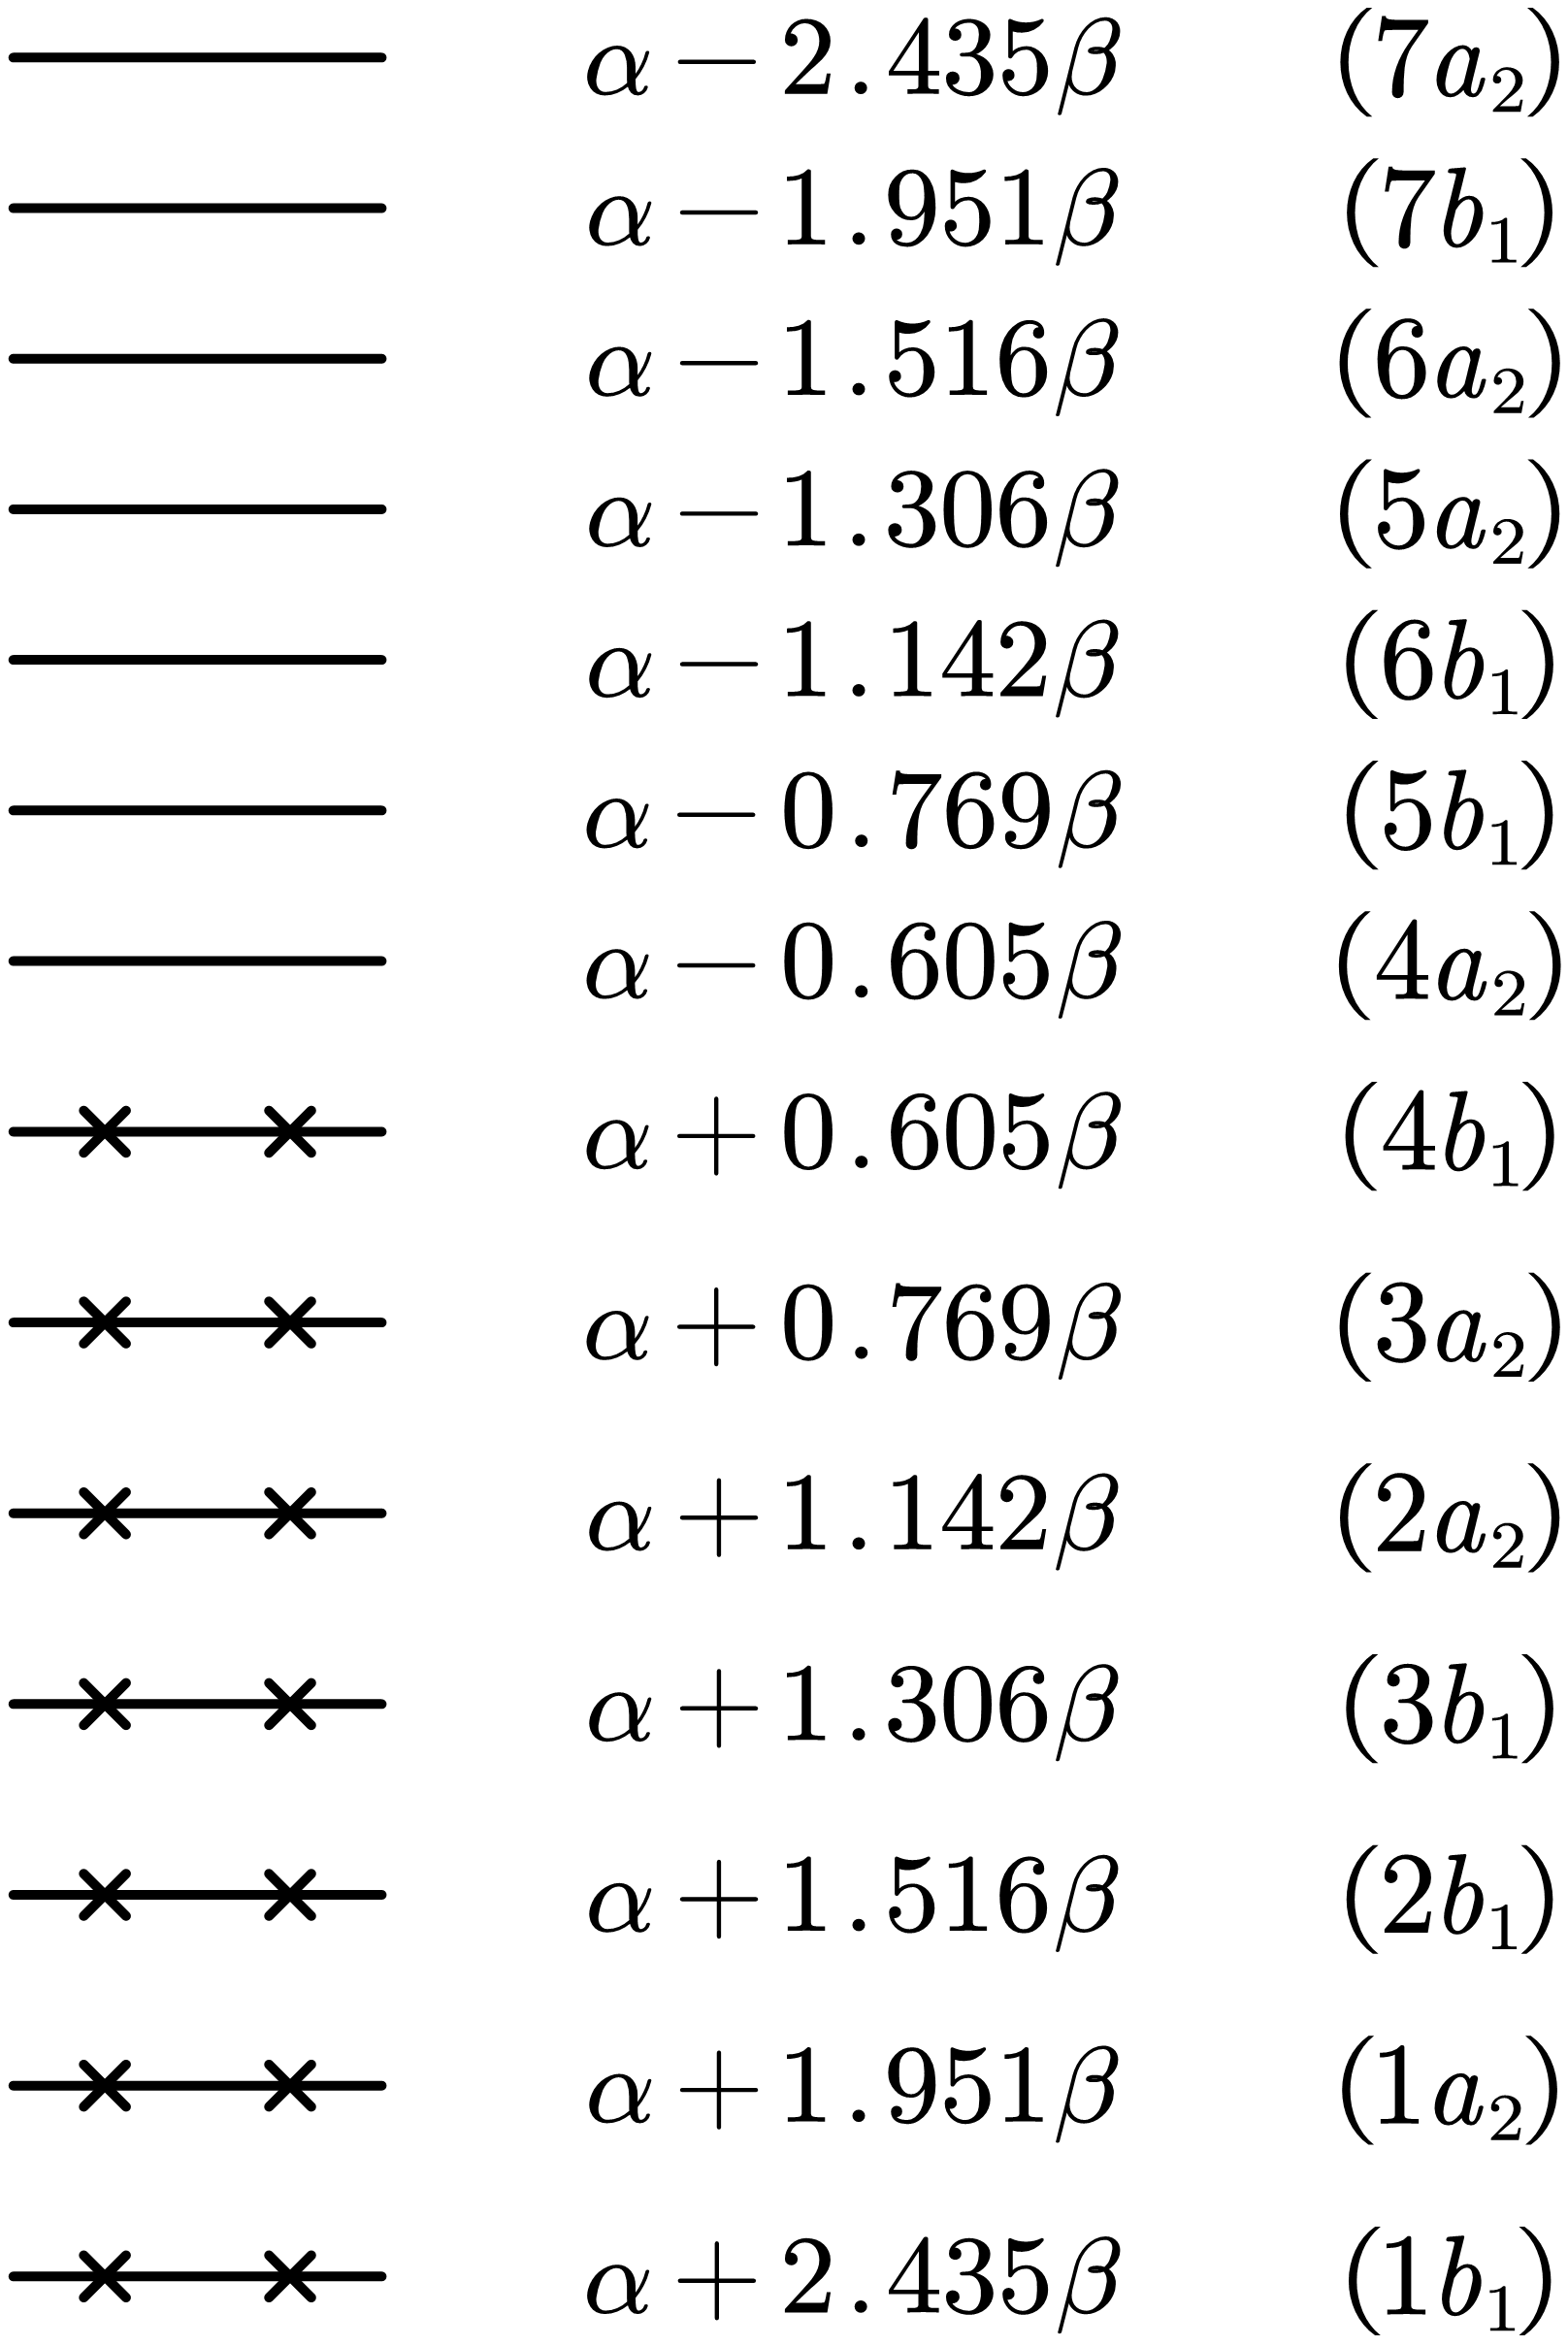
\includegraphics[scale=1.0]{./structures/exercise_1/phenanthrene/998.png}
		\end{center}